\documentclass[12pt,]{article}
\usepackage{lmodern}
\usepackage{amssymb,amsmath}
\usepackage{ifxetex,ifluatex}
\usepackage{fixltx2e} % provides \textsubscript
\ifnum 0\ifxetex 1\fi\ifluatex 1\fi=0 % if pdftex
  \usepackage[T1]{fontenc}
  \usepackage[utf8]{inputenc}
\else % if luatex or xelatex
  \ifxetex
    \usepackage{mathspec}
  \else
    \usepackage{fontspec}
  \fi
  \defaultfontfeatures{Ligatures=TeX,Scale=MatchLowercase}
    \setmainfont[]{Helvetica}
\fi
% use upquote if available, for straight quotes in verbatim environments
\IfFileExists{upquote.sty}{\usepackage{upquote}}{}
% use microtype if available
\IfFileExists{microtype.sty}{%
\usepackage{microtype}
\UseMicrotypeSet[protrusion]{basicmath} % disable protrusion for tt fonts
}{}
\usepackage{hyperref}
\hypersetup{unicode=true,
            pdftitle={Biogeography \& Environmental Conditions Shape Phage \& Bacteria Interaction Networks Across the Human Microbiome},
            pdfborder={0 0 0},
            breaklinks=true}
\urlstyle{same}  % don't use monospace font for urls
\usepackage{graphicx,grffile}
\makeatletter
\def\maxwidth{\ifdim\Gin@nat@width>\linewidth\linewidth\else\Gin@nat@width\fi}
\def\maxheight{\ifdim\Gin@nat@height>\textheight\textheight\else\Gin@nat@height\fi}
\makeatother
% Scale images if necessary, so that they will not overflow the page
% margins by default, and it is still possible to overwrite the defaults
% using explicit options in \includegraphics[width, height, ...]{}
\setkeys{Gin}{width=\maxwidth,height=\maxheight,keepaspectratio}
\IfFileExists{parskip.sty}{%
\usepackage{parskip}
}{% else
\setlength{\parindent}{0pt}
\setlength{\parskip}{6pt plus 2pt minus 1pt}
}
\setlength{\emergencystretch}{3em}  % prevent overfull lines
\providecommand{\tightlist}{%
  \setlength{\itemsep}{0pt}\setlength{\parskip}{0pt}}
\setcounter{secnumdepth}{0}
% Redefines (sub)paragraphs to behave more like sections
\ifx\paragraph\undefined\else
\let\oldparagraph\paragraph
\renewcommand{\paragraph}[1]{\oldparagraph{#1}\mbox{}}
\fi
\ifx\subparagraph\undefined\else
\let\oldsubparagraph\subparagraph
\renewcommand{\subparagraph}[1]{\oldsubparagraph{#1}\mbox{}}
\fi
\usepackage{setspace}
\doublespacing
\usepackage[vmargin=1in,hmargin=1in]{geometry}
\usepackage{lineno}
\linenumbers
\usepackage{parskip}
\setlength{\parskip}{7.5pt}
\exhyphenpenalty=10000
\hyphenpenalty=10000

\newcommand{\beginsupplement}{%
        \setcounter{table}{0}
        \renewcommand{\thetable}{S\arabic{table}}%
        \setcounter{figure}{0}
        \renewcommand{\thefigure}{S\arabic{figure}}%
     }

\title{Biogeography \& Environmental Conditions Shape Phage \& Bacteria
Interaction Networks Across the Human Microbiome}
    \usepackage{authblk}
    \font\myfont=Helvetica at 12pt
    \font\nextfont=Helvetica at 10pt
                        \author[1]{\myfont Geoffrey D Hannigan}
                    \author[2]{\myfont Melissa B Duhaime}
                    \author[3]{\myfont Danai Koutra}
                    \author[1,*]{\myfont Patrick D Schloss}
                            \affil[1]{\nextfont Department of Microbiology \& Immunology, University of Michigan, Ann
Arbor, Michigan, 48109}
                    \affil[2]{\nextfont Department of Ecology \& Evolutionary Biology, University of Michigan,
Ann Arbor, Michigan, 48109}
                    \affil[3]{\nextfont Department of Computer Science, University of Michigan, Ann Arbor,
Michigan, 48109}
                    \affil[*]{\nextfont To whom correspondence may be addressed.}
            \date{}

\begin{document}
\maketitle

~

~

~

\textbf{\emph{Running Title}}: Network Diversity of the Healthy Human
Microbiome

\textbf{\emph{Corresponding Author Information}}\\
Patrick D Schloss, PhD\\
1150 W Medical Center Dr.~1526 MSRB I\\
Ann Arbor, Michigan 48109\\
Phone: (734) 647-5801\\
Email: pschloss@umich.edu

\newpage

\section{Abstract}\label{abstract}

Viruses and bacteria are critical components of the human microbiome and
play important roles in health and disease. Most previous work has
relied on studying microbes and viruses independently, thereby reducing
them to two separate communities. Such approaches are unable to capture
how these microbial communities interact, such as through processes that
maintain community stability or allow phage-host populations to
co-evolve. We developed and implemented a network-based analytical
approach to describe phage-bacteria network diversity throughout the
human body. We accomplished this by building a machine learning
algorithm to predict which phages could infect which bacteria in a given
microbiome. This algorithm was applied to paired viral and bacterial
metagenomic sequence sets from three previously published human cohorts.
We organized the predicted interactions into networks that allowed us to
evaluate phage-bacteria connectedness across the human body. We found
that gut and skin network structures were person-specific and not
conserved among cohabitating family members. High-fat diets and obesity
were associated with less connected networks. Network structure differed
between skin sites, with those exposed to the external environment being
less connected and more prone to instability. This study quantified and
contrasted the diversity of virome-microbiome networks across the human
body and illustrated how environmental factors may influence
phage-bacteria interactive dynamics. This work provides a baseline for
future studies to better understand system perturbations, such as
disease states, through ecological networks.

\newpage

\section{Importance}\label{importance}

The human microbiome, the collection of microbial communities that
colonize the human body, is a crucial component to health and disease.
Two major components to the human microbiome are the bacterial and viral
communities. These communities have primarily been studied separately
using metrics of community composition and diversity. These approaches
have failed to capture the complex dynamics of interacting bacteria and
phage communities, which frequently share genetic information and work
together to maintain stable ecosystems. Removal of bacteria or phage can
disrupt or even collapse those ecosystems. Relationship-based network
approaches allow us to capture this interaction information. Using this
network-based approach with three independent human cohorts, we were
able to present an initial understanding of how phage-bacteria networks
differ throughout the human body, so as to provide a baseline for future
studies of how and why microbiome networks differ in disease states.

\newpage

\section{Introduction}\label{introduction}

Viruses and bacteria are critical components of the human microbiome and
play important roles in health and disease. Bacterial communities have
been associated with disease states, including a range of skin
conditions {[}1{]}, acute and chronic wound healing conditions
{[}2,3{]}, and gastrointestinal diseases, such as inflammatory bowel
disease {[}4,5{]}, \emph{Clostridium difficile} infections {[}6{]} and
colorectal cancer {[}7,8{]}. Altered human viromes (virus communities
consisting primarily of bacteriophages) also have been associated with
diseases and perturbations, including inflammatory bowel disease
{[}5,9{]}, periodontal disease {[}10{]}, spread of antibiotic resistance
{[}11{]}, and others {[}12--17{]}. Viruses act in concert with their
microbial hosts as a single ecological community {[}18{]}. Viruses
influence their living microbial host communities through processes
including lysis, host gene expression modulation {[}19{]}, influence on
evolutionary processes such as horizontal gene transfer {[}22{]} or
antagonistic co-evolution {[}26{]}, and alteration of ecosystem
processes and elemental stoichiometry {[}27{]}.

Previous human microbiome work has focused on bacterial and viral
communities, but have reduced them to two separate communities by
studying them independently {[}5,9,10,12--17{]}. This approach fails to
capture the complex dynamics of interacting bacteria and phage
communities, which frequently share genetic information and work
together to maintain stable ecosystems. Removal of bacteria or phage can
disrupt or even collapse those ecosystems {[}18,28--37{]}.
Relationship-based network approaches allow us to capture this
interaction information. Studying such bacteria-phage interactions
through community-wide networks built from inferred relationships could
offer further insights into the drivers of human microbiome diversity
across body sites and enable the study of human microbiome network
dynamics overall.

In this study, we characterized human-associated bacterial and phage
communities by their inferred relationships using three published paired
virus and bacteria-dominated whole community metagenomic datasets
{[}13,14,38,39{]}. We leveraged machine learning and graph theory
techniques to establish and explore the human bacteria-phage network
diversity therein. This approach built upon previous large-scale
phage-bacteria network analyses by inferring interactions from
metagenomic datasets, rather than culture-dependent data {[}33{]}, which
is limited in the scale of possible experiments and analyses. Our
metagenomic interaction inference model improved upon previous models of
phage-host predictions that have utilized a variety of techniques, such
as linear models to predict bacteria-phage co-occurrence using taxonomic
assignments {[}40{]}, and nucleotide similarity models that were applied
to both whole virus genomes {[}41{]} and related clusters of whole and
partial virus genomes {[}42{]}. Our approach uniquely included protein
interaction data and was validated based on experimentally determined
positive and negative interactions (i.e.~who does and does not infect
whom). Through this approach we were able to provide a basic
understanding of the network dynamics associated with phage and
bacterial communities on and in the human body. By building and
utilizing a microbiome network, we found that different people, body
sites, and anatomical locations not only support distinct microbiome
membership and diversity {[}13,14,38,39,43--45{]}, but also support
ecological communities with distinct communication structures and
propensities toward community instability. Through an improved
understanding of network structures across the human body, we empower
future studies to investigate how these communities dynamics are
influenced by disease states and the overall impact they may have on
human health.

\section{Results}\label{results}

\subsection{Cohort Curation and Sample
Processing}\label{cohort-curation-and-sample-processing}

We studied the differences in virus-bacteria interaction networks across
healthy human bodies by leveraging previously published shotgun sequence
datasets of purified viral metagenomes (viromes) paired with
bacteria-dominated whole community metagenomes. Our study contained
three datasets that explored the impact of diet on the healthy human gut
virome {[}14{]}, the impact of anatomical location on the healthy human
skin virome {[}13{]}, and the viromes of monozygotic twins and their
mothers {[}38,39{]}. We selected these datasets because their virome
samples were subjected to virus-like particle (VLP) purification. To
this end, they employed combinations of filtration, chloroform/DNase
treatment, and cesium chloride gradients to eliminate organismal DNA and
thereby allow for direct assessment of both the extracellular and
fully-assembled intracellular virome \textbf{(Supplemental Figure
\ref{SequenceStats} A-B)} {[}14,39{]}. While the whole metagenomic
shotgun sequence samples were not subjected to purification, they
primarily consisted of bacteria {[}13,14,38,39{]}.

The bacterial and viral sequences from these studies were quality
filtered and assembled into contigs. We further grouped the related
bacterial and phage contigs into operationally defined units based on
their k-mer frequencies and co-abundance patterns, similar to previous
reports \textbf{(Supplemental Figure \ref{ContigStats} -
\ref{ClusterStats})} {[}42{]}. We referred to these operationally
defined groups of related contigs as operational genomic units (OGUs).
Each OGU represented a genomically similar sub-population of either
bacteria or phages. Contig lengths within clusters ranged between
\(10^{3}\) and \(10^{5.5}\) bp \textbf{(Supplemental Figure
\ref{ContigStats} - \ref{ClusterStats})}.

\subsection{Evaluating the Model to Predict Phage-Bacteria
Interactions}\label{evaluating-the-model-to-predict-phage-bacteria-interactions}

We predicted which phage OGUs infected which bacterial OGUs using a
random forest model trained on experimentally validated infectious
relationships from six previous publications {[}41,47--51{]}. Only
bacteria and phages were used in the model. The training set contained
43 diverse bacterial species and 30 diverse phage strains, including
both broad and specific ranges of infection \textbf{(Supplemental Figure
\ref{ValidationOverview} A - B)}. Phages with linear and circular
genomes, as well as ssDNA and dsDNA genomes, were included in the
analysis. Because we used DNA sequencing studies, RNA phages were not
considered \textbf{(Supplemental Figure \ref{ValidationOverview} C-D)}.
This training set included both positive relationships (a phage infects
a bacterium) and negative relationships (a phage does not infect a
bacterium). This allowed us to validate the false positive and false
negative rates associated with our candidate models, thereby building
upon previous work that only considered positive relationships {[}41{]}.

Four phage and bacterial genomic features were used in a random forest
model to predict infectious relationships between bacteria and phages:
1) genome nucleotide similarities, 2) gene amino acid sequence
similarities, 3) bacterial Clustered Regularly Interspaced Short
Palindromic Repeat (CRISPR) spacer sequences that target phages, and 4)
similarity of protein families associated with experimentally identified
protein-protein interactions {[}52{]}. The resulting random forest model
was assessed and the area under its receiver operating characteristic
(ROC) curve was 0.846, the model sensitivity was 0.829, and specificity
was 0.767 \textbf{(Figure \ref{RocCurve} A)}. The most important
predictor in the model was amino acid similarity between genes, followed
by nucleotide similarity of whole genomes \textbf{(Figure \ref{RocCurve}
B)}. Protein family interactions were moderately important to the model,
and CRISPRs were largely uninformative, due to the minimal amount of
identifiable CRISPRs in the dataset and their redundancy with the
nucleotide similarity methods \textbf{(Figure \ref{RocCurve} B)}.
Approximately one third of the training set relationships yielded no
score and therefore were unable to be assigned an interaction prediction
\textbf{(Figure \ref{RocCurve} C)}.

We used our random forest model to classify the relationships between
bacteria and phage operational genomic units, which were then used to
build the interactive network. The master network contained the three
studies as sub-networks, which themselves each contained sub-networks
for each sample \textbf{(Figure \ref{RocCurve} D)}. Metadata including
study, sample ID, disease, and OGU abundance within the community were
stored in the master network for parsing in downstream analyses
\textbf{(Supplemental Figure \ref{NetworkDiagram})}. The master network
was highly connected and contained 72,287 infectious relationships among
578 nodes, representing 298 phages and 280 bacteria. Although the
network was highly connected, not all relationships were present in all
samples. As relationships were weighted by the relative abundances of
their associated bacteria and phages, lowly abundant relationships could
be present but not highly abundant. Like the master network, the skin
network exhibited a diameter of 4 (measure of graph size; the greatest
number of traversed vertices required between two vertices) and included
99.7\% and 99.8\% of the master network nodes and edges, respectively
\textbf{(Figure \ref{RocCurve} E - F)}. The phages and bacteria in the
gut diet and twin sample sets were more sparsely related: each contained
fewer than 150 vertices, fewer than 20,000 relationships, and diameters
of 3 \textbf{(Figure \ref{RocCurve} E - F)}.

\subsection{Role of Diet \& Obesity in Gut Microbiome
Connectivity}\label{role-of-diet-obesity-in-gut-microbiome-connectivity}

Diet is a major environmental factor that influences resource
availability and gut microbiome composition and diversity, including
bacteria and phages {[}14,53,54{]}. Previous work in isolated
culture-based systems has suggested that changes in nutrient
availability are associated with altered phage-bacteria network
structures {[}30{]}, although this has yet to be tested in humans. We
therefore hypothesized that a change in diet would also be associated
with a change in virome-microbiome network structure in the human gut.

We evaluated the diet-associated differences in gut virome-microbiome
network structure by quantifying how central each sample's network was
on average. We accomplished this by utilizing two common centrality
metrics: degree centrality and closeness centrality. Degree centrality,
the simplest centrality metric, was defined as the number of connections
each phage made with each bacterium. We supplemented measurements of
degree centrality with measurements of closeness centrality. Closeness
centrality is a metric of how close each phage or bacterium is to all of
the other phages and bacteria in the network. A higher closeness
centrality suggests that the effects of genetic information or altered
abundance would be more impactful to all other microbes in the system. A
network with higher average closeness centrality also indicates an
overall greater degree of connections, which suggests a greater
resilience against instability. We used this information to calculate
the average connectedness per sample, which was corrected for the
maximum potential degree of connectedness.

We found that the gut microbiome network structures associated with
high-fat diets were less connected than those of low-fat diets
\textbf{(Figure \ref{dietnetworks} A-B)}. Tests for statistical
differences were not performed due to the small sample size. High-fat
diets exhibited reduced degree centrality \textbf{(Figure
\ref{dietnetworks} A)}, suggesting bacteria in high-fat environments
were targeted by fewer phages and that phage tropism was more
restricted. High-fat diets also exhibited decreased closeness centrality
\textbf{(Figure \ref{dietnetworks} B)}, indicating that bacteria and
phages were more distant from other bacteria and phages in the
community. This would make genetic transfer and altered abundance of a
given phage or bacterium less capable of impacting other bacteria and
phages within the network.

In addition to diet, obesity was found to influence network structure.
Obesity-associated networks demonstrated a higher degree centrality
\textbf{(Figure \ref{dietnetworks} C)}, but less closeness centrality
than the healthy-associated networks \textbf{(Figure \ref{dietnetworks}
D)}. These results suggested that the obesity-associated networks are
less connected, having microbes further from all other microbes within
the community.

\subsection{Individuality of Microbial
Networks}\label{individuality-of-microbial-networks}

Skin and gut community membership and diversity are highly personal,
with people remaining more similar to themselves than to other people
over time {[}13,55,56{]}. We therefore hypothesized that this personal
conservation extended to microbiome network structure. We addressed this
hypothesis by calculating the degree of dissimilarity between each
subject's network, based on phage and bacteria abundance and centrality.
We quantified phage and bacteria centrality within each sample graph
using the weighted eigenvector centrality metric. This metric defines
central phages as those that are highly abundant (\(A_{O}\) as defined
in the methods) and infect many distinct bacteria which themselves are
abundant and infected by many other phages. Similarly, bacterial
centrality was defined as those bacteria that were both abundant and
connected to numerous phages that were themselves connected to many
bacteria. We then calculated the similarity of community networks using
the weighted eigenvector centrality of all nodes between all samples.
Samples with similar network structures were interpreted as having
similar capacities for maintaining stability and transmitting genetic
material.

We used this network dissimilarity metric to test whether microbiome
network structures were more similar within people than between people
over time. We found that gut microbiome network structures clustered by
person (ANOSIM p-value = 0.005, R = 0.958, \textbf{Figure \ref{intradiv}
A}). Network dissimilarity within each person over the 8-10 day sampling
period was less than the average dissimilarity between that person and
others, although this difference was not statistically significant
(p-value = 0.125, \textbf{Figure \ref{intradiv} B}). The lack of
statistical confidence was likely due to the small sample size of this
dataset. Although there was evidence for gut network conservation among
individuals, we found no evidence for conservation of gut network
structures within families. The gut network structures were not more
similar within families (twins and their mothers; intrafamily) compared
to other families (inter-family) (p-value = 0.312, \textbf{Figure
\ref{intradiv} C}). In addition to the gut, skin microbiome network
structure was strongly conserved within individuals (p-value \textless{}
0.001, \textbf{Figure \ref{intradiv} D}). This distribution was similar
when separated by anatomical sites. Most sites were statistically
significantly more conserved within individuals \textbf{(Supplemental
Figure \ref{allskin})}.

\subsection{Association Between Environmental Stability and Network
Structure Across the Human Skin
Landscape}\label{association-between-environmental-stability-and-network-structure-across-the-human-skin-landscape}

Extensive work has illustrated differences in diversity and composition
of the healthy human skin microbiome between anatomical sites, including
bacteria, virus, and fungal communities {[}13,44,55{]}. These
communities vary by degree of skin moisture, oil, and environmental
exposure. As viruses are known to influence microbial diversity and
community composition, we hypothesized that microbe-virus network
structure would be specific to anatomical sites, as well. To test this,
we evaluated the changes in network structure between anatomical sites
within the skin dataset.

The average centrality of each sample was quantified using the weighted
eigenvector centrality metric. Intermittently moist skin sites (dynamic
sites that fluctuate between being moist and dry) were significantly
less connected than the more stable moist and sebaceous environments
(p-value \textless{} 0.001, \textbf{Figure \ref{skinnetwork} A)}. Also,
skin sites that were occluded from the environment were much more highly
connected than those that were constantly exposed to the environment or
only intermittently occluded (p-value \textless{} 0.001, \textbf{Figure
\ref{skinnetwork} B)}.

To supplement this analysis, we compared the network signatures using
the centrality dissimilarity approach described above. The dissimilarity
between samples was a function of shared relationships, degree of
centrality, and bacteria/phage abundance. When using this supplementary
approach, we found that network structures significantly clustered by
moisture, sebaceous, and intermittently moist status \textbf{(Figure
\ref{skinnetwork} C,E)}. Occluded sites were significantly different
from exposed and intermittently occluded sites, but there was no
difference between exposed and intermittently occluded sites
\textbf{(Figure \ref{skinnetwork} D,F)}. These findings provide further
support that skin microbiome network structure differs significantly
between skin sites.

\section{Discussion}\label{discussion}

Foundational work has provided a baseline understanding of the human
microbiome by characterizing bacterial and viral diversity across the
human body {[}13,14,43--45,57{]}. Here, we offer an initial
understanding of how phage-bacteria networks differ throughout the human
body, so as to provide a baseline for future studies of how and why
microbiome networks differ in disease states. We developed and
implemented a network-based analytical model to evaluate the basic
properties of the human microbiome through bacteria and phage
relationships, instead of membership or diversity alone. This enabled
the application of network theory to provide a new perspective on
complex ecological communities. We utilized metrics of connectivity to
model the extent to which communities of bacteria and phages interact
through mechanisms such as horizontal gene transfer, modulated bacterial
gene expression, and alterations in abundance.

Just as gut microbiome and virome composition and diversity are
conserved in individuals {[}13,43,44,56{]}, gut and skin microbiome
network structures were conserved within individuals over time. Gut
network structure was not conserved among family members. These findings
suggested that the community properties inferred from microbiome
interaction network structures, such as stability, the potential for
horizontal gene transfer between members, and co-evolution of
populations, were person-specific. These properties may be impacted by
personal factors ranging from the body's immune system to external
environmental conditions, such as climate and diet.

The ability of environmental conditions to shape gut and skin microbiome
interaction network structure was further supported by our finding that
diet and skin location were associated with altered network structures.
We found evidence that diet was sufficient to alter gut microbiome
network connectivity. Although our sample size was small, our findings
provided evidence that high-fat diets were less connected than low-fat
diets and that high-fat diets therefore may lead to less stable
communities with a decreased ability for microbes to directly influence
one another. We supported this finding with the observation that obesity
may have been associated with decreased network connectivity. Together
these findings suggest the food we eat may not only impact which
microbes colonize our guts, but may also impact their interactions with
infecting phages. Further work will be required to characterize these
relationships with a larger cohort.

In addition to diet, the skin environment also influenced the microbiome
interaction network structure. Network structure differed between
environmentally exposed and occluded skin sites. The sites under greater
environmental fluctuation and exposure (the exposed and intermittently
exposed sites) were less connected and therefore were predicted to have
a higher propensity for instability. Likewise, intermittently moist
sites demonstrated less connectedness than the more stable moist and
sebaceous sites. Together these data suggested that body sites under
greater degrees of fluctuation harbored less connected, potentially less
stable microbiomes. This points to a link between microbiome and
environmental stability and warrants further investigation.

While these findings take us an important step closer to understanding
the microbiome through interspecies relationships, there are caveats to
and considerations regarding the approach. First, as with most
classification models, the infection classification model developed and
applied is only as good as its training set -- in this case, the
collection of experimentally-verified positive and negative infection
data, where genomes of all members are fully sequenced. Large-scale
experimental screens for phage and bacteria infectious interactions that
report high-confidence negative interactions (i.e., no infection) are
desperately needed, as they would provide more robust model training and
improved model performance. Furthermore, just as we have improved on
previous modeling efforts, we expect that new and creative scoring
metrics will be integrated into this model to improve future
performance.

Second, although our analyses utilized the best datasets currently
avilable for our study, this work was done retrospectively and relied on
existing data up to seven years old. These archived datasets were
limited by the technology and costs of the time. For example, the diet
and twin studies, relied on multiple displacement amplification (MDA) in
their library preparations--an approach used to overcome the large
nucleic acids requirements typical of older sequencing library
generation protocols. It is now known that MDA results in biases in
microbial community composition {[}58{]}, as well as toward ssDNA viral
genomes {[}59,60{]}, thus rendering the resulting microbial and viral
metagenomes largely non-quantitative. Future work that employs larger
sequence datasets and that avoids the use of bias-inducing amplification
steps will build on and validate our findings, as well as inform the
design and interpretation of further studies.

Finally, the networks in this study were built using operational genomic
units (OGUs), which represented groups of highly similar bacteria or
phage genomes or genome fragments as clustered sub-populations. Similar
clustering definition and validation methods, both computational and
experimental, have been implemented in other metagenomic sequencing
studies, as well {[}42,61--63{]}. These approaches could offer yet
another level of sophistication to our network-based analyses. While
this operationally defined clustering approach allows us to study whole
community networks, our ability to make conclusions about interactions
among specific phage or bacterial species or populations is inherently
limited. Future work must address this limitation, e.g., through
improved binning methods and deeper metagenomic shotgun sequencing, but
most importantly through an improved conceptual framing of what defines
ecologically and evolutionarily cohesive units for both phage and
bacteria {[}64{]}. Defining operational genomic units and their
taxonomic underpinnings (e.g., whether OGU clusters represent genera or
species) is an active area of work critical to the utility of this
approach. As a first step, phylogenomic analyses have been performed to
cluster cyanophage isolate genomes into informative groups using shared
gene content, average nucleotide identity of shared genes, and pairwise
differences between genomes {[}65{]}. Such population-genetic assessment
of phage evolution, coupled with the ecological implications of genome
heterogeneity, will inform how to define nodes in future iterations of
the ecological network developed here.

Together our work takes an initial step towards defining bacteria-virus
interaction profiles as a characteristic of human-associated microbial
communities. This approach revealed the impacts that different human
environments (e.g., the skin and gut) can have on microbiome
connectivity. By focusing on relationships between bacterial and viral
communities, they are studied as the interacting cohorts they are,
rather than as independent entities. While our developed bacteria-phage
interaction framework is a novel conceptual advance, the microbiome also
consists of archaea and small eukaryotes, including fungi and
\emph{Demodex} mites {[}1,66{]}--all of which can interact with human
immune cells and other non-microbial community members {[}67{]}. Future
work will build from our approach and include these additional community
members and their diverse interactions and relationships (e.g., beyond
phage-bacteria). This will result in a more robust network and a more
holistic understanding of the evolutionary and ecological processes that
drive the assembly and function of the human-associated microbiome.

\section{Materials \& Methods}\label{materials-methods}

\subsection{Code Availability}\label{code-availability}

A reproducible version of this manuscript written in R markdown and all
of the code used to obtain and process the sequencing data is available
at the following GitHub repository:

https://github.com/SchlossLab/Hannigan\_ConjunctisViribus\_mSystems\_2017

\subsection{Data Acquisition \& Quality
Control}\label{data-acquisition-quality-control}

Raw sequencing data and associated metadata were acquired from the NCBI
sequence read archive (SRA). Supplementary metadata were acquired from
the same SRA repositories and their associated manuscripts. The gut
virome diet study (SRA: \texttt{SRP002424}), twin virome studies (SRA:
\texttt{SRP002523}; \texttt{SRP000319}), and skin virome study (SRA:
\texttt{SRP049645}) were downloaded as \texttt{.sra} files. Sequencing
files were converted to \texttt{fastq} format using the
\texttt{fastq-dump} tool of the NCBI SRA Toolkit (v2.2.0). Sequences
were quality trimmed using the Fastx toolkit (v0.0.14) to exclude bases
with quality scores below 33 and shorter than 75 bp {[}68{]}. Paired end
reads were filtered to exclude sequences missing their corresponding
pair using the \texttt{get\_trimmed\_pairs.py} script available in the
source code.

\subsection{Contig Assembly}\label{contig-assembly}

Contigs were assembled using the Megahit assembly program (v1.0.6)
{[}69{]}. A minimum contig length of 1 kb was used. Iterative k-mer
stepping began at a minimum length of 21 and progressed by 20 until 101.
All other default parameters were used.

\subsection{Contig Abundance
Calculations}\label{contig-abundance-calculations}

Contigs were concatenated into two master files prior to alignment, one
for bacterial contigs and one for phage contigs. Sample sequences were
aligned to phage or bacterial contigs using the Bowtie2 global aligner
(v2.2.1) {[}70{]}. We defined a mismatch threshold of 1 bp and seed
length of 25 bp. Sequence abundance was calculated from the Bowtie2
output using the \texttt{calculate\_abundance\_from\_sam.pl} script
available in the source code.

\subsection{Operational Genomic Unit
Binning}\label{operational-genomic-unit-binning}

Contigs often represent large fragments of genomes. In order to reduce
redundancy and the resulting artificially inflated genomic richness
within our dataset, it was important to bin contigs into operational
units based on their similarity. This approach is conceptually similar
to the clustering of related 16S rRNA sequences into operational
taxonomic units (OTUs), although here we are clustering contigs into
operational genomic units (OGUs) {[}57{]}.

Contigs were clustered using the CONCOCT algorithm (v0.4.0) {[}71{]}.
Because of our large dataset and limits in computational efficiency, we
randomly subsampled the dataset to include 25\% of all samples, and used
these to inform contig abundance within the CONCOCT algorithm. CONCOCT
was used with a maximum of 500 clusters, a k-mer length of four, a
length threshold of 1 kb, 25 iterations, and exclusion of the total
coverage variable.

OGU abundance (\(A_{O}\)) was obtained as the sum of the abundance of
each contig (\(A_{j}\)) associated with that OGU. The abundance values
were length corrected such that:

\[ { A }_{ O }=\frac { { 10 }^{ 7 }\sum _{ j=1 }^{ k }{ { A }_{ j } }  }{ \sum _{ j=1 }^{ k }{ { L }_{ j } }  } \]

Where \texttt{L} is the length of each contig \texttt{j} within the OGU.

\subsection{Phage OGU Identification}\label{phage-ogu-identification}

To confirm a lack of phage sequences in the bacterial OGU dataset, we
performed blast nucleotide alignment of the bacterial OGU representative
sequences using an e-value \textless{} \(10^{-25}\), which was stricter
than the \(10^{-10}\) threshold used in the random forest model below.
We used a stricter threshold because we know there are genomic
similarities between bacteria and phage OGUs from the interactive model,
but we were interested in contigs with high enough similarity to
references that they may indeed be from phages. 2\% of the OGUs had
nucleotide similarities to known bacteriophage genomes, although the
alignments were short (a couple of kb) and represented a small fraction
of the alignment sequences.

\subsection{Open Reading Frame
Prediction}\label{open-reading-frame-prediction}

Open reading frames (ORFs) were identified using the Prodigal program
(V2.6.2) with the meta mode parameter and default settings {[}72{]}.

\subsection{Classification Model Creation and
Validation}\label{classification-model-creation-and-validation}

The classification model for predicting interactions was built using
experimentally validated bacteria-phage infections or validated lack of
infections from six studies {[}41,47--51{]}. Associated reference
genomes were downloaded from the European Bioinformatics Institute (see
details in source code). The model was created based on the four metrics
listed below.

The four scores were used as parameters in a random forest model to
classify bacteria and bacteriophage pairs as either having infectious
interactions or not. The classification model was built using the Caret
R package (v6.0.73) {[}73{]}. The model was trained using five-fold
cross validation with ten repeats. Pairs without scores were classified
as not interacting. The model was optimized using the ROC value. The
resulting model performance was plotted using the plotROC R package.

\subparagraph{Identify Bacterial CRISPRs Targeting
Phages}\label{identify-bacterial-crisprs-targeting-phages}

Clustered Regularly Interspaced Short Palindromic Repeats (CRISPRs) were
identified from bacterial genomes using the PilerCR program (v1.06)
{[}74{]}. Resulting spacer sequences were filtered to exclude spacers
shorter than 20 bp and longer than 65 bp. Spacer sequences were aligned
to the phage genomes using the nucleotide BLAST algorithm with default
parameters (v2.4.0) {[}75{]}. The mean percent identity for each
matching pair was recorded for use in our classification model.

\subparagraph{Detect Matching Prophages within Bacterial
Genomes}\label{detect-matching-prophages-within-bacterial-genomes}

Temperate bacteriophages infect and integrate into their bacterial
host's genome. We detected integrated phage elements within bacterial
genomes by aligning phage genomes to bacterial genomes using the
nucleotide BLAST algorithm and a minimum e-value of 1e-10. The resulting
bitscore of each alignment was recorded for use in our classification
model.

\subparagraph{Identify Shared Genes Between Bacteria and
Phages}\label{identify-shared-genes-between-bacteria-and-phages}

As a result of gene transfer or phage genome integration during
infection, phages may share genes with their bacterial hosts, providing
us with evidence of phage-host pairing. We identified shared genes
between bacterial and phage genomes by assessing amino acid similarity
between the genes using the Diamond protein alignment algorithm
(v0.7.11.60) {[}76{]}. The mean alignment bitscores for each genome pair
were recorded for use in our classification model.

\subparagraph{Protein - Protein
Interactions}\label{protein---protein-interactions}

The final method used for predicting infectious interactions between
bacteria and phages was the detection of pairs of genes whose proteins
are known to interact. We assigned bacterial and phage genes to protein
families by aligning them to the Pfam database using the Diamond protein
alignment algorithm. We then identified which pairs of proteins were
predicted to interact using the Pfam interaction information within the
Intact database {[}52{]}. The mean bitscores of the matches between each
pair were recorded for use in the classification model.

\subsection{Interaction Network
Construction}\label{interaction-network-construction}

The bacteria and phage operational genomic units (OGUs) were scored
using the same approach as outlined above. The infectious pairings
between bacteria and phage OGUs were classified using the random forest
model described above. The predicted infectious pairings and all
associated metadata were used to populate a graph database using Neo4j
graph database software (v2.3.1) {[}77{]}. This network was used for
downstream community analysis.

\subsection{Centrality Analysis}\label{centrality-analysis}

We quantified the centrality of graph vertices using three different
metrics, each of which provided different information graph structure.
When calculating these values, let \(G(V,E)\) be an undirected,
unweighted graph with \(|V|=n\) nodes and \(|E|=m\) edges. Also, let
\(\mathbf{A}\) be its corresponding adjacency matrix with entries
\(a_{ij} = 1\) if nodes \(V_i\) and \(V_j\) are connected via an edge,
and \(a_{ij} = 0\) otherwise.

Briefly, the \textbf{closeness centrality} of node \(V_i\) is calculated
taking the inverse of the average length of the shortest paths
(\texttt{d}) between nodes \(V_i\) and all the other nodes \(V_j\).
Mathematically, the closeness centrality of node \(V_i\) is given as:

\[ { C }_{ C }\left( { V }_{ i } \right) ={ \left( \sum _{ j=1 }^{ n }{ d\left( { V }_{ i },{ V }_{ j } \right)  }  \right)  }^{ -1 } \]

The distance between nodes (\texttt{d}) was calculated as the shortest
number of edges required to be traversed to move from one node to
another.

Intuitively, the \textbf{degree centrality} of node \(V_i\) is defined
as the number of edges that are incident to that node:

\[ { C }_{ D }\left( { V }_{ i } \right) =\sum _{ j=1 }^{ n }{ { a }_{ ij } } \]

where \(a_{ij}\) is the \(ij^{th}\) entry in the adjacency matrix
\(\mathbf{A}\).

The eigenvector centrality of node \(V_i\) is defined as the \(i^{th}\)
value in the first eigenvector of the associated adjacency matrix
\(\mathbf{A}\). Conceptually, this function results in a centrality
value that reflects the connections of the vertex, as well as the
centrality of its neighboring vertices.

The \textbf{centralization} metric was used to assess the average
centrality of each sample graph \(\mathbf{G}\). Centralization was
calculated by taking the sum of each vertex \(V_{i}\)'s centrality from
the graph maximum centrality \(C_{w}\), such that:

\[ C\left( G \right) =\frac { \sum _{ i=1 }^{ n }{ Cw -c\left( { V }_{ i } \right)  }  }{ { T } }  \]

The values were corrected for uneven graph sizes by dividing the
centralization score by the maximum theoretical centralization
(\texttt{T}) for a graph with the same number of vertices.

Degree and closeness centrality were calculated using the associated
functions within the igraph R package (v1.0.1) {[}78{]}.

\subsection{Network Relationship
Dissimilarity}\label{network-relationship-dissimilarity}

We assessed similarity between graphs by evaluating the shared
centrality of their vertices, as has been done previously. More
specifically, we calculated the dissimilarity between graphs \(G_{i}\)
and \(G_{j}\) using the Bray-Curtis dissimilarity metric and eigenvector
centrality values such that:

\[ B\left( { G }_{ i },{ G }_{ j } \right) =1-\frac { 2{ C }_{ ij } }{ { C }_{ i }+{ C }_{ j } } \]

Where \(C_{ij}\) is the sum of the lesser centrality values for those
vertices shared between graphs, and \(C_{i}\) and \(C_{j}\) are the
total number of vertices found in each graph. This allows us to
calculate the dissimilarity between graphs based on the shared
centrality values between the two graphs.

\subsection{Statistics and
Comparisons}\label{statistics-and-comparisons}

Differences in intrapersonal and interpersonal network structure
diversity, based on multivariate data, were calculated using an analysis
of similarity (ANOSIM). Statistical significance of univariate
Eigenvector centrality differences were calculated using a paired
Wilcoxon test.

Statistical significance of differences in univariate eigenvector
centrality measurements of skin virome-microbiome networks were
calculated using a pairwise Wilcoxon test, corrected for multiple
hypothesis tests using the Holm correction method. Multivariate
eigenvector centrality was measured as the mean differences between
cluster centroids, with statistical significance measured using an ANOVA
and post hoc Tukey test.

\section{Acknowledgments}\label{acknowledgments}

We thank the members of the Schloss lab for their underlying
contributions.

\section{Funding Information}\label{funding-information}

GDH was supported in part by the Molecular Mechanisms in Microbial
Pathogenesis Training Program (T32 AI007528). GDH and PDS were supported
in part by funding from the NIH (P30DK034933, U19AI09087, and
U01AI124255).

\section{Disclosure Declaration}\label{disclosure-declaration}

The authors report no conflicts of interest.

\newpage

\section{Figures}\label{figures}

\begin{figure}[htbp]
\centering
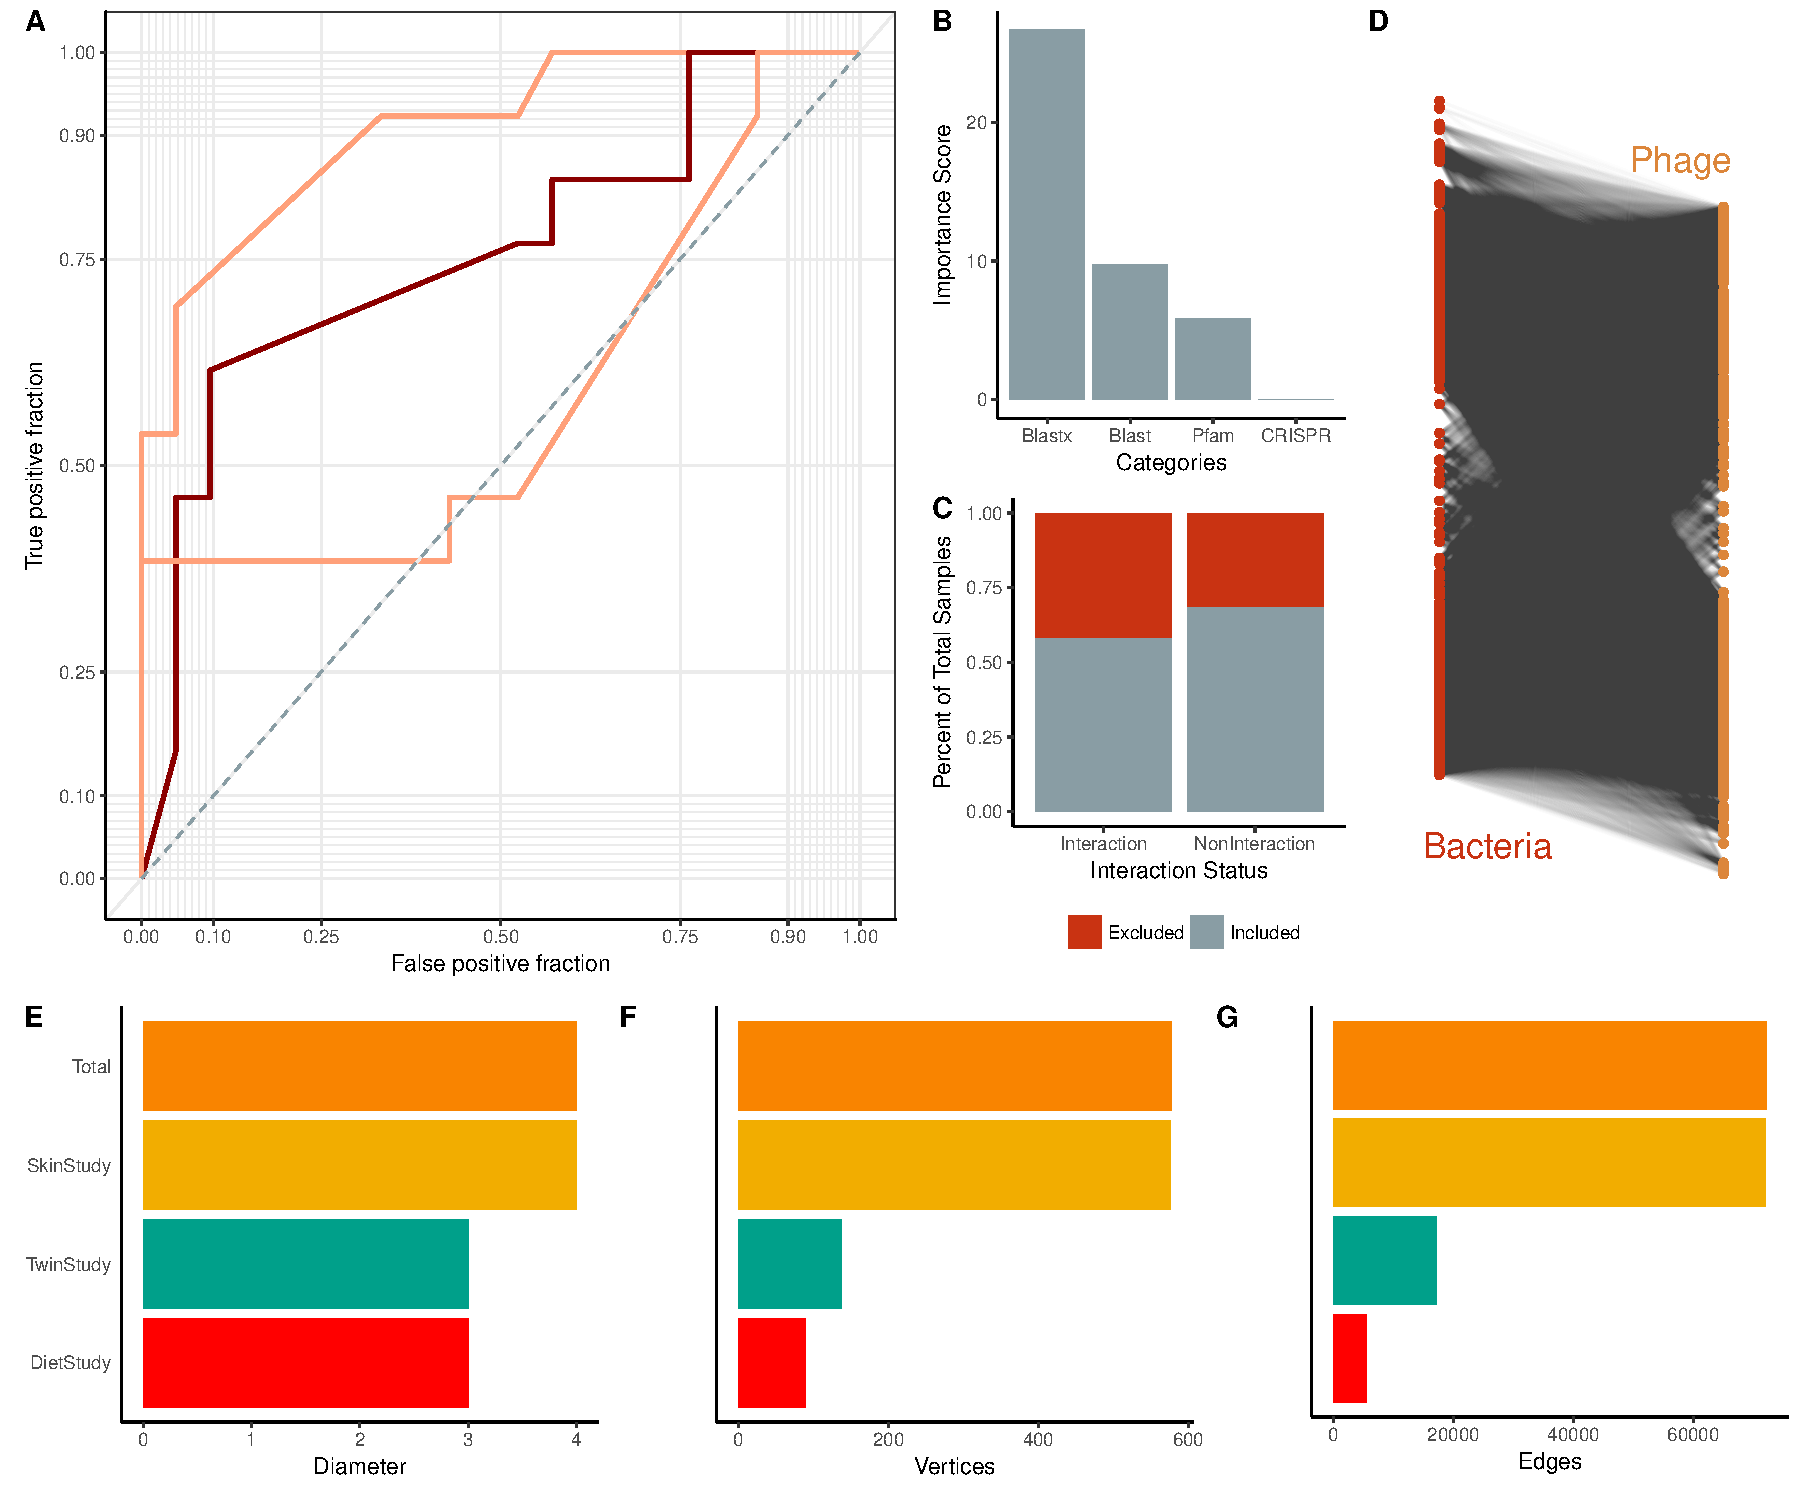
\includegraphics[width=0.85000\textwidth]{../figures/rocCurves.pdf}
\caption{\textbf{Summary of Multi-Study Network Model.} \emph{(A)
Average ROC curve used to create the microbiome-virome infection
prediction model. (B) Importance scores associated with the metrics used
in the random forest model to predict relationships between bacteria and
phages. The importance score is defined as the mean decrease in accuracy
of the model when a feature (e.g.~Pfam) is excluded. (C) Proportions of
samples included (gray) and excluded (red) in the model. Samples were
excluded from the model because they did not yield any scores. Those
interactions without scores were defined as not having interactions. (D)
Bipartite visualization of the resulting phage-bacteria network. This
network includes information from all three published studies. (E)
Network diameter (measure of graph size; the greatest number of
traversed vertices required between two vertices), (F) number of
vertices, and (G) number of edges (relationships) for the total network
(yellow) and the individual study sub-networks (diet study = red, skin
study = green, twin study = orange).} \label{RocCurve}}
\end{figure}

\newpage

\begin{figure}[htbp]
\centering
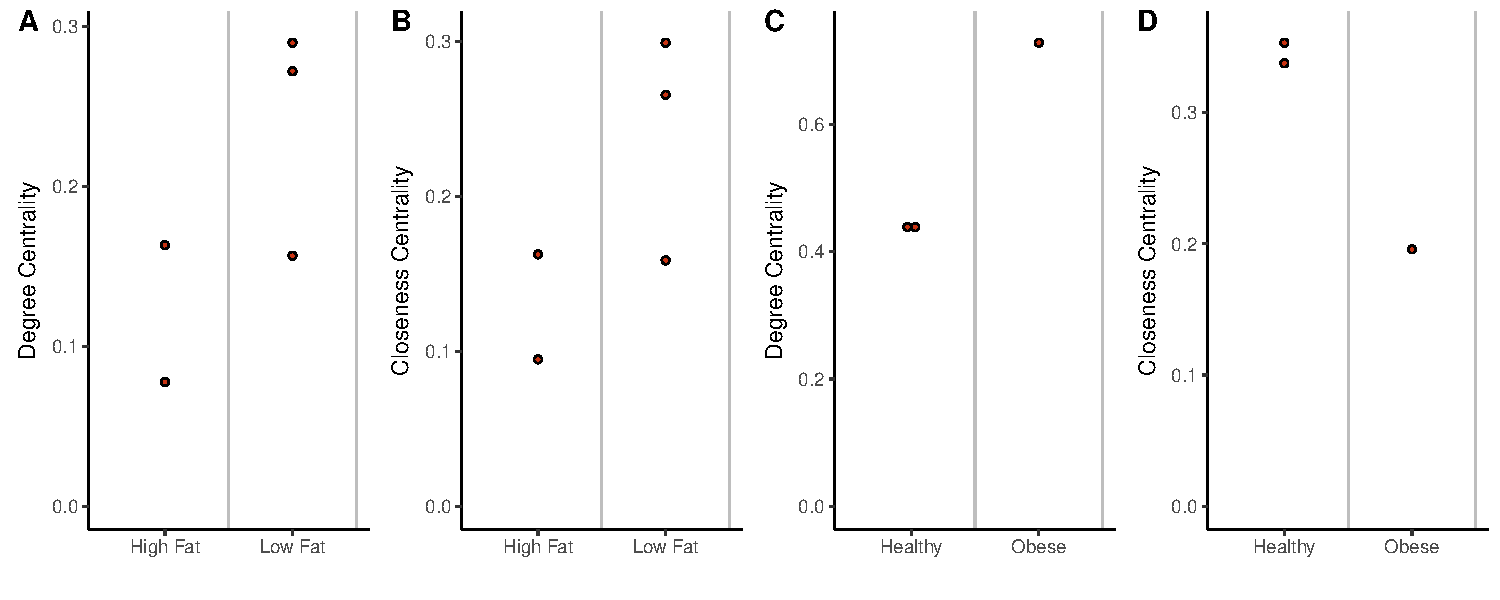
\includegraphics[width=0.90000\textwidth]{../figures/dietnetworks.pdf}
\caption{\textbf{Impact of Diet and Obesity on Gut Network Structure.}
\emph{(A) Quantification of average degree centrality (number of edges
per node) and (B) closeness centrality (average distance from each node
to every other node) of gut microbiome networks of subjects limited to
exclusively high-fat or low-fat diets. Lines represent the mean degree
of centrality for each diet. (C) Quantification of average degree
centrality and (D) closeness centrality between obese and healthy adult
women.}\label{dietnetworks}}
\end{figure}

\newpage

\begin{figure}[htbp]
\centering
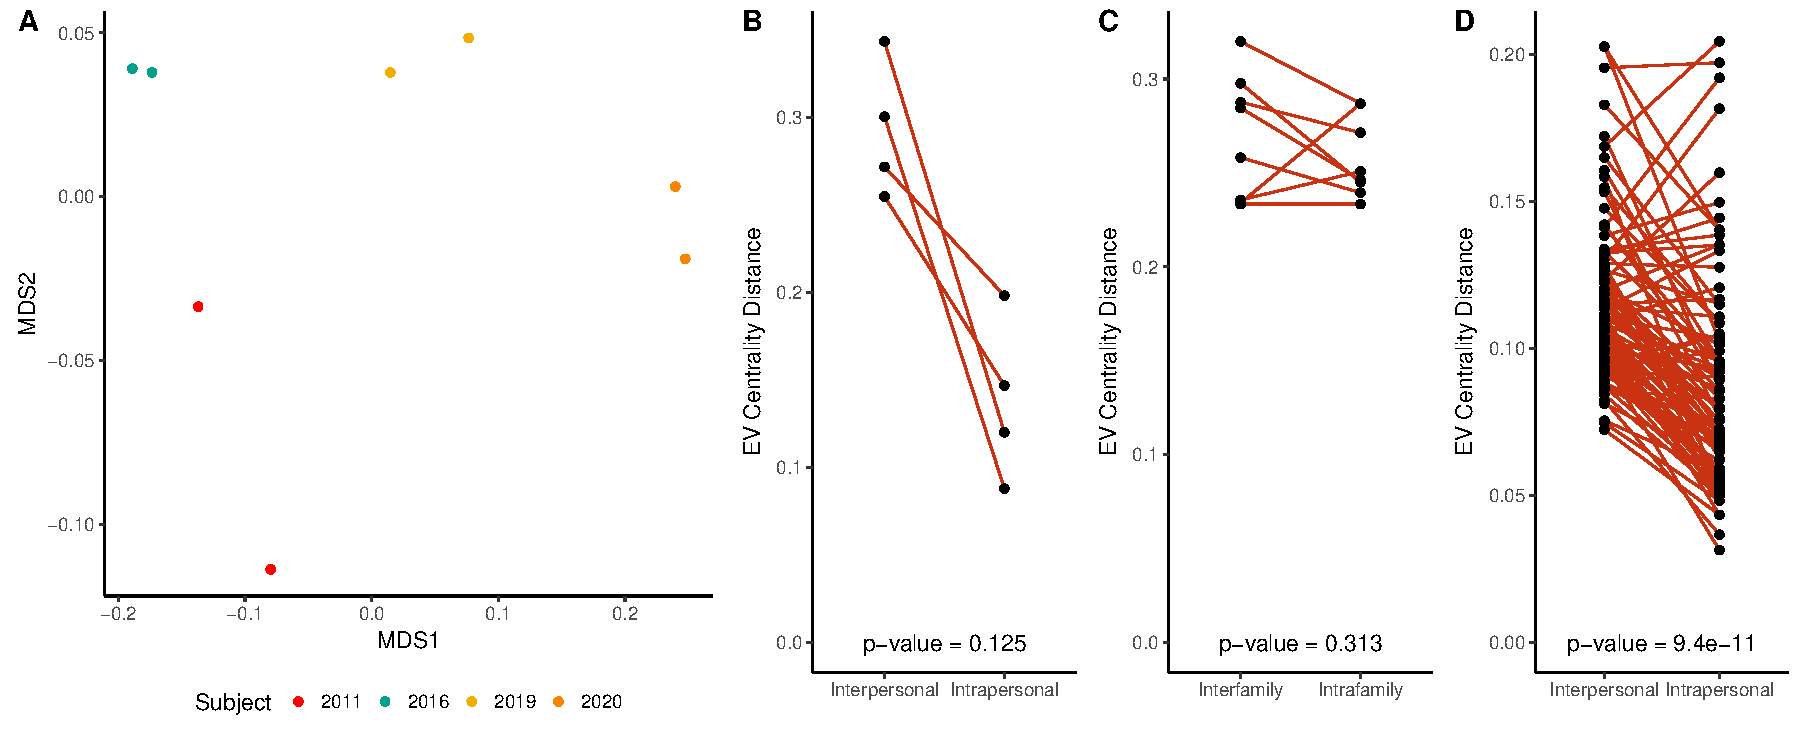
\includegraphics[width=0.90000\textwidth]{../figures/intrapersonal_diversity.pdf}
\caption{\textbf{Intrapersonal vs Interpersonal Network Dissimilarity
Across Different Human Systems.} \emph{(A) NMDS ordination illustrating
network dissimilarity between subjects over time. Each sample is colored
by subject, with each sample pair collected 8-10 days apart.
Dissimilarity was calculated using the Bray-Curtis metric based on
abundance weighted eigenvector centrality signatures, with a greater
distance representing greater dissimilarity in bacteria and phage
centrality and abundance. (B) Quantification of gut network
dissimilarity within the same subject over time (intrapersonal) and the
mean dissimilarity between the subject of interest and all other
subjects (interpersonal). The p-value is also provided. (C)
Quantification of gut network dissimilarity within subjects from the
same family (intrafamily) and the mean dissimilarity between subjects
within a family and those of other families (interfamily). The p-value
is also provided. (D) Quantification of skin network dissimilarity
within the same subject and anatomical location over time
(intrapersonal) and the mean dissimilarity between the subject of
interest and all other subjects at the same time and the same anatomical
location (interpersonal). P-value was calculated using a paired Wilcoxon
test.}\label{intradiv}}
\end{figure}

\begin{figure}[htbp]
\centering
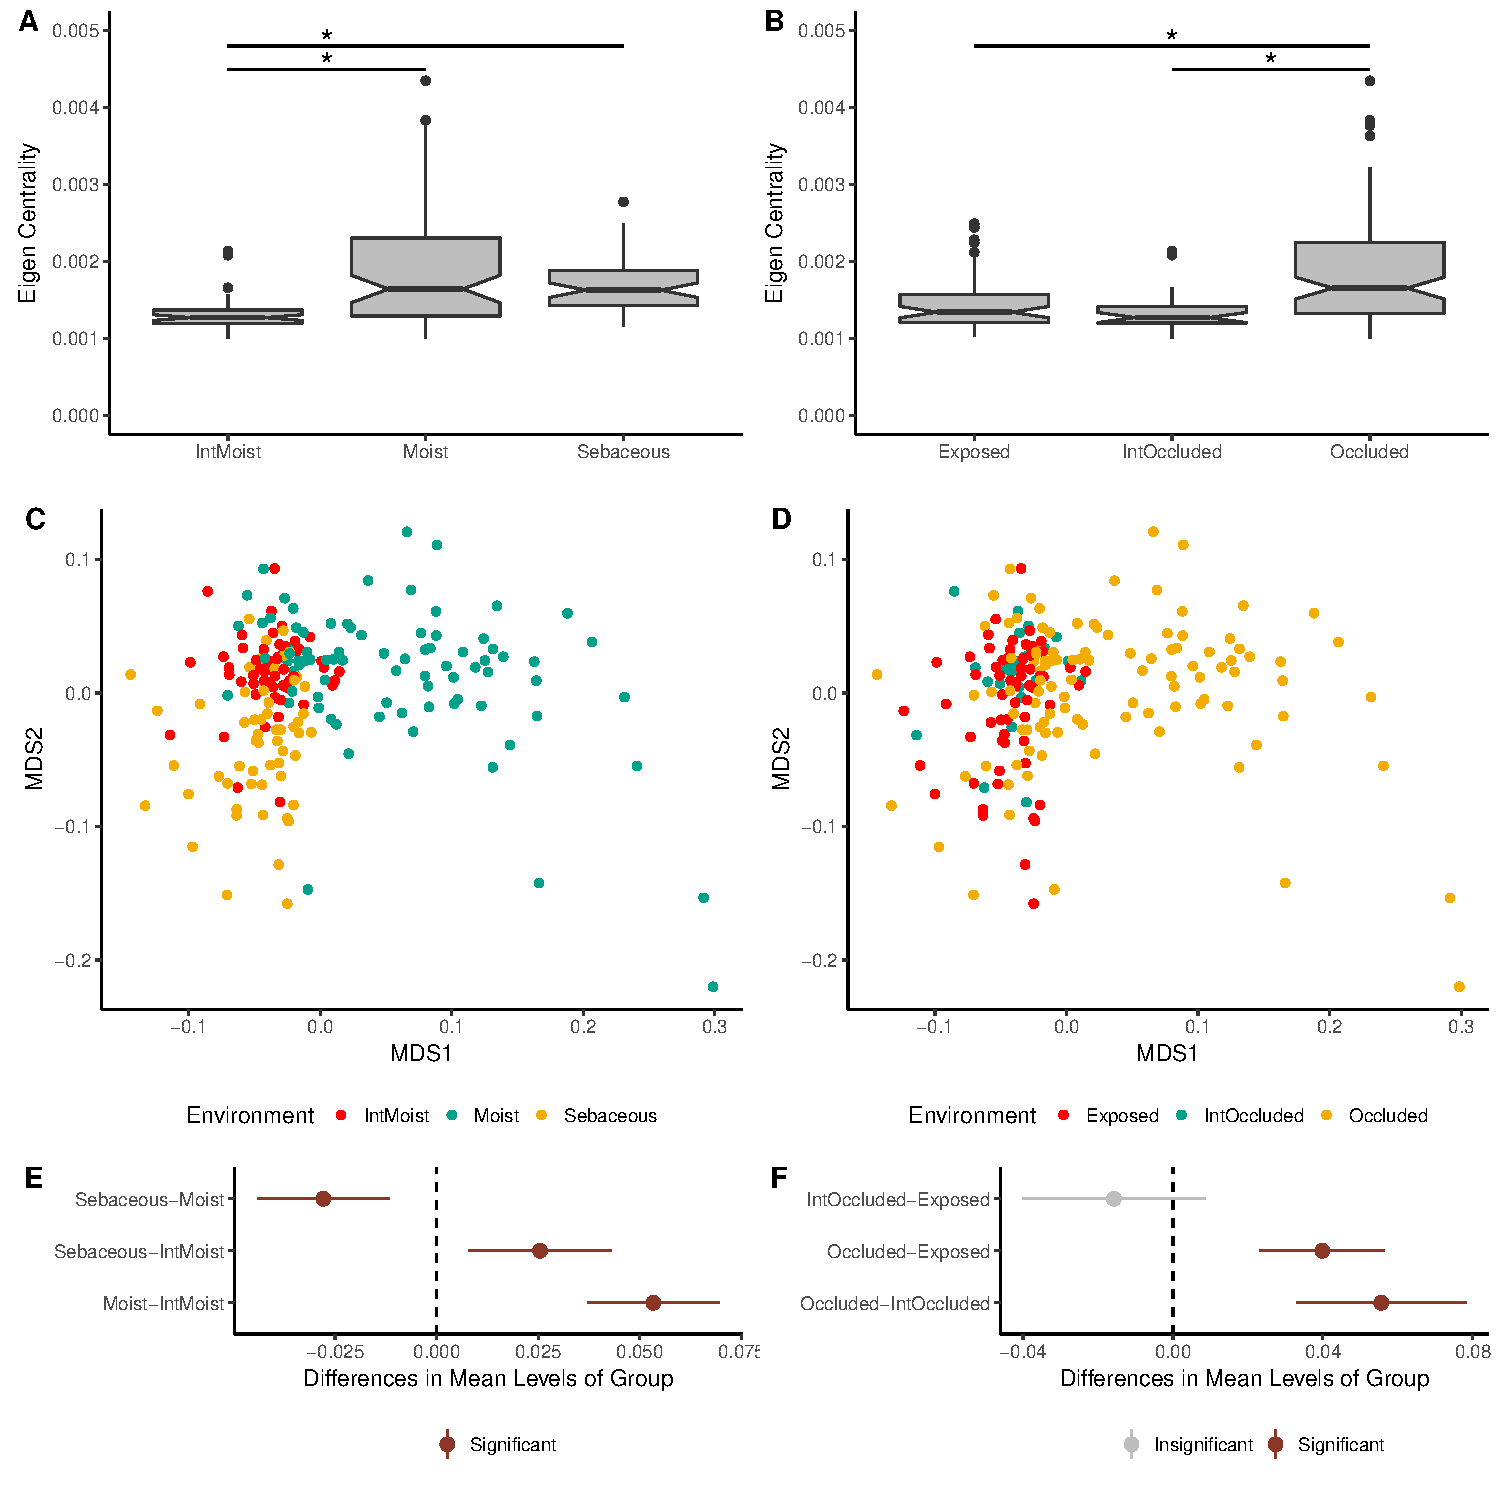
\includegraphics[width=0.75000\textwidth]{../figures/skinplotresults.pdf}
\caption{\textbf{Impact of Skin Micro-Environment on Microbiome Network
Structure.} \emph{(A) Notched box-plot depicting differences in average
eigenvector centrality between moist, intermittently moist, and
sebaceous skin sites and (B) occluded, intermittently occluded, and
exposed sites. Notched box-plots were created using ggplot2 and show the
median (center line), the inter-quartile range (IQR; upper and lower
boxes), the highest and lowest value within 1.5 * IQR (whiskers),
outliers (dots), and the notch which provides an approximate 95\%
confidence interval as defined by 1.58 * IQR / sqrt(n). (C) NMDS
ordination depicting the differences in skin microbiome network
structure between skin moisture levels and (D) occlusion. Samples are
colored by their environment and their dissimilarity to other samples
was calculated as described in figure \ref{intradiv}. (E) The
statistical differences of networks between moisture and (F) occlusion
status were quantified with an anova and post hoc Tukey test. Cluster
centroids are represented by dots and the extended lines represent the
associated 95\% confidence intervals. Significant comparisons (p-value
\textless{} 0.05) are colored in red, and non-significant comparisons
are gray.}\label{skinnetwork}}
\end{figure}

\newpage

\section{Supplemental Figures}\label{supplemental-figures}

\beginsupplement

\begin{figure}[htbp]
\centering
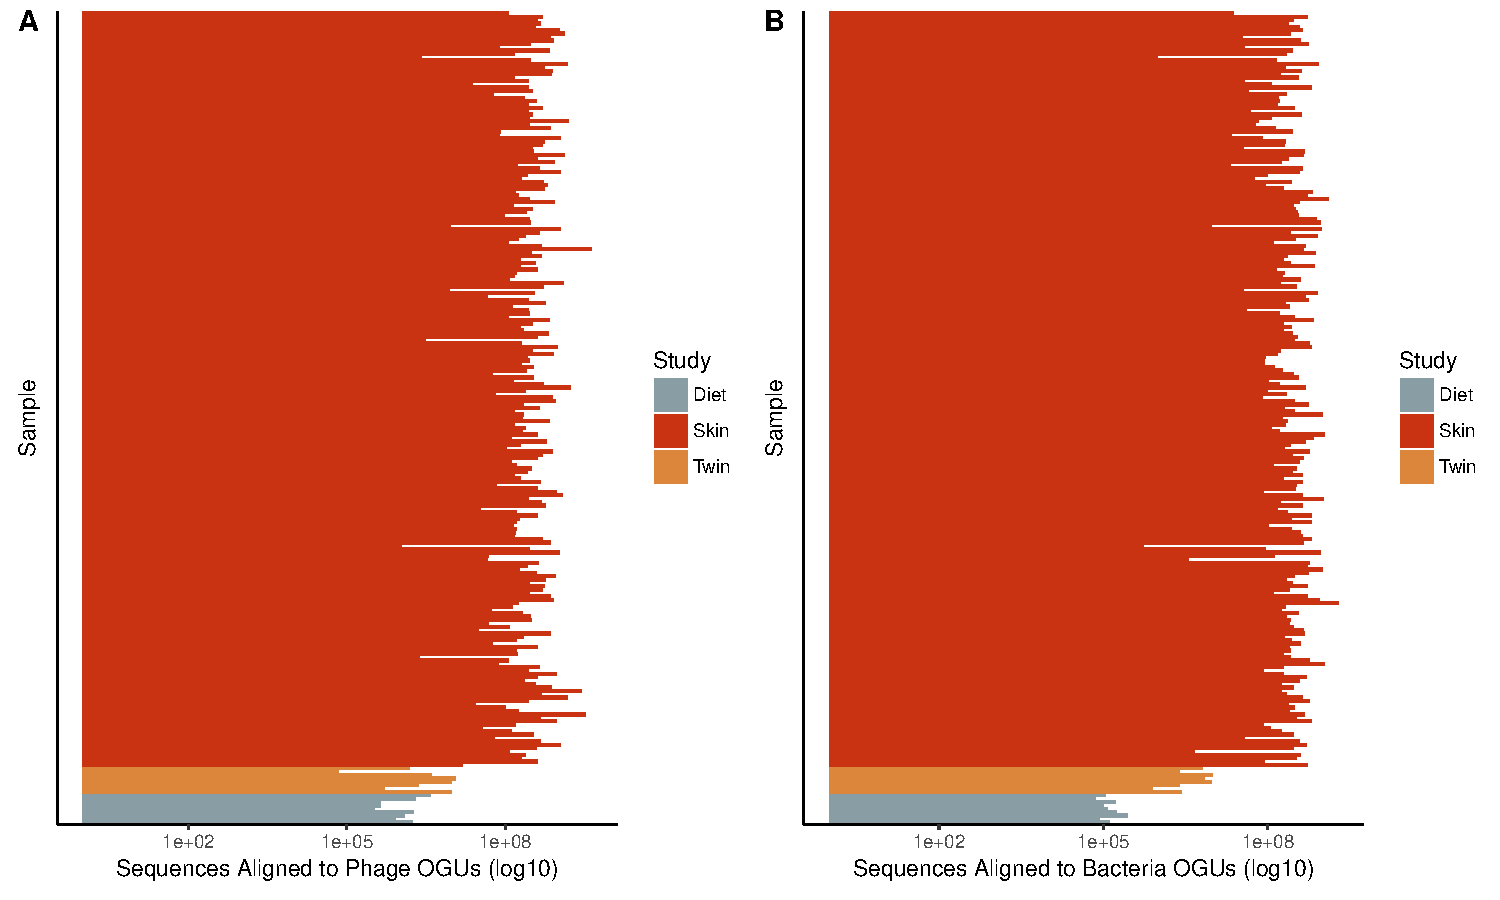
\includegraphics[width=0.80000\textwidth]{../figures/SequenceAbund.pdf}
\caption{\textbf{Sequencing Depth Summary.} \emph{Number of sequences
that aligned to (A) Phage and (B) Bacteria operational genomic units per
sample and colored by study.}\label{SequenceStats}}
\end{figure}

\newpage

\begin{figure}[htbp]
\centering
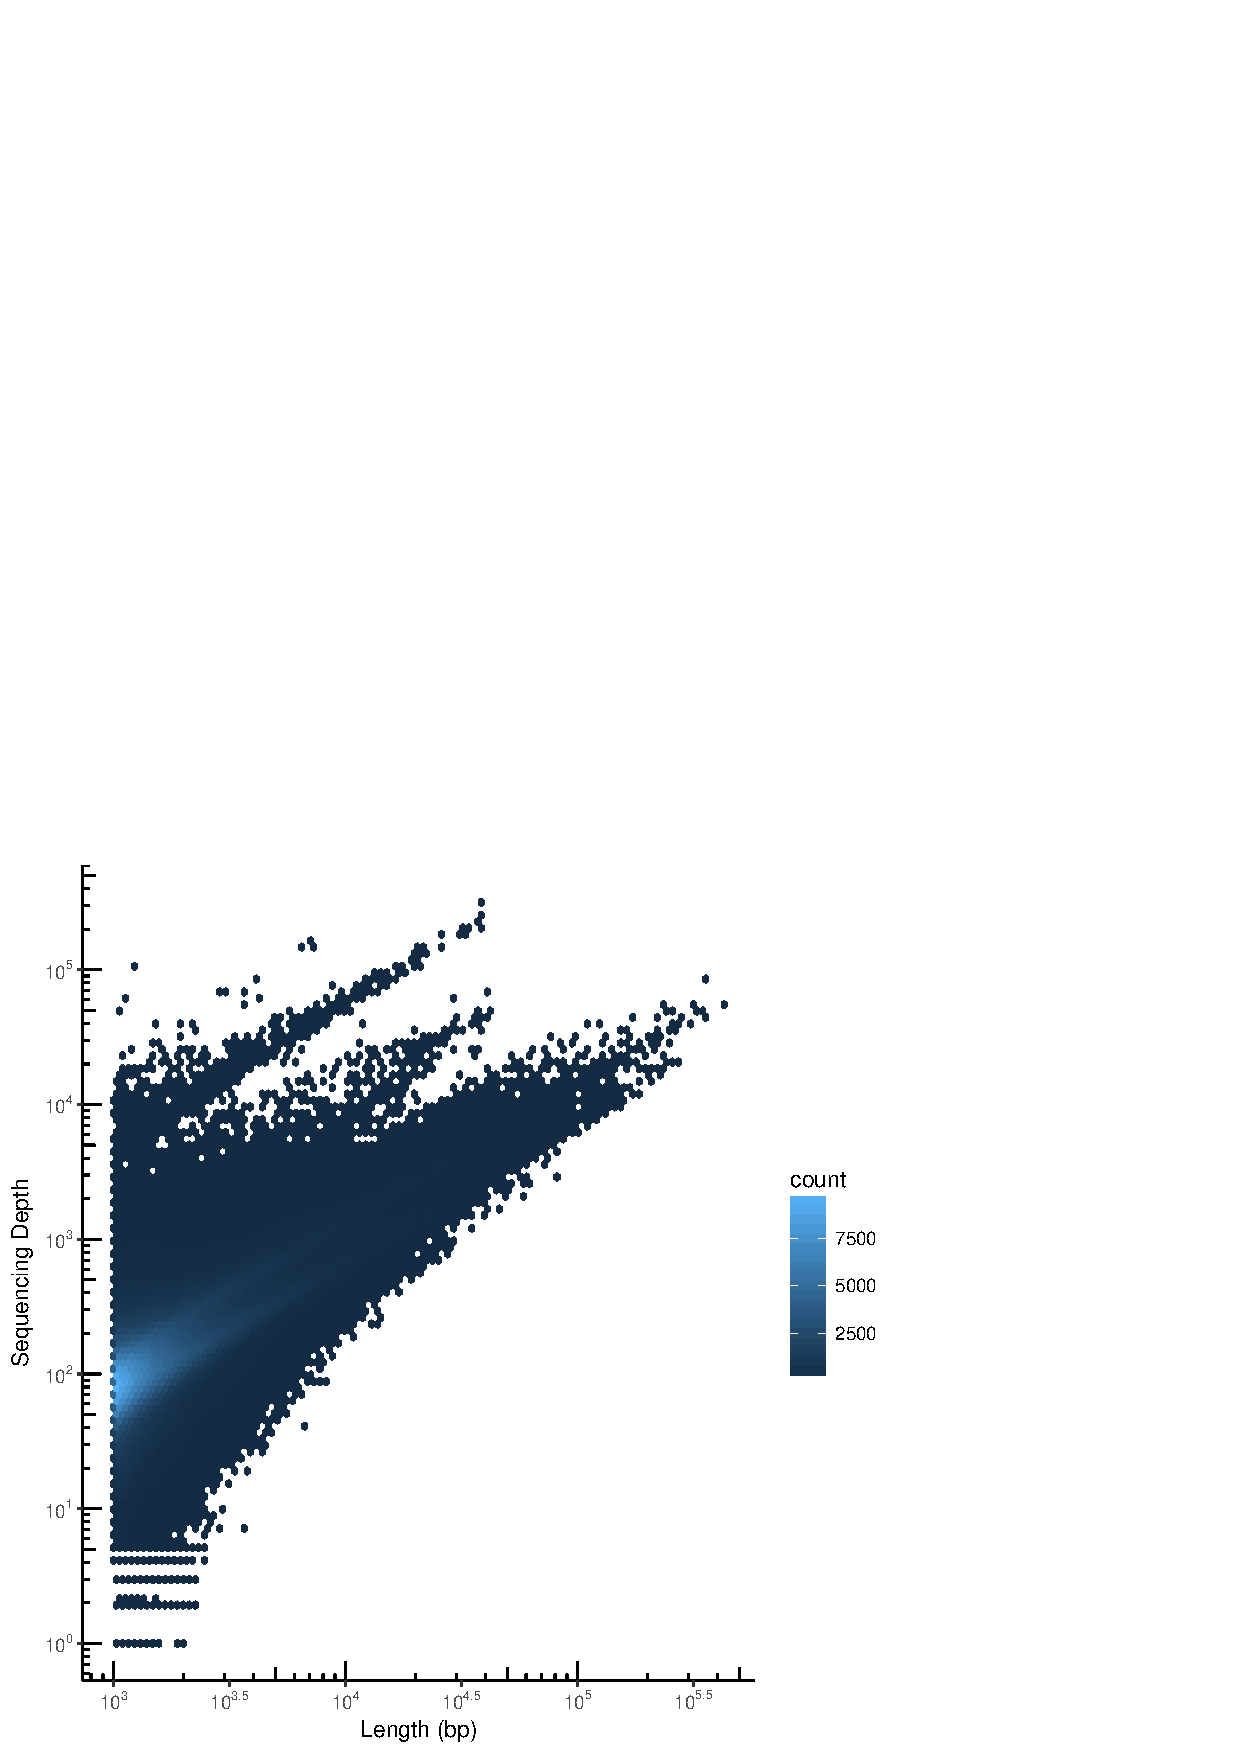
\includegraphics[width=0.50000\textwidth]{../figures/ContigStats.pdf}
\caption{\textbf{Contig Summary Statistics.} \emph{Scatter plot heat map
with each hexagon representing the abundance of contigs. Contigs are
organized by length on the x-axis and the number of aligned sequences on
the y-axis.}\label{ContigStats}}
\end{figure}

\newpage

\begin{figure}[htbp]
\centering
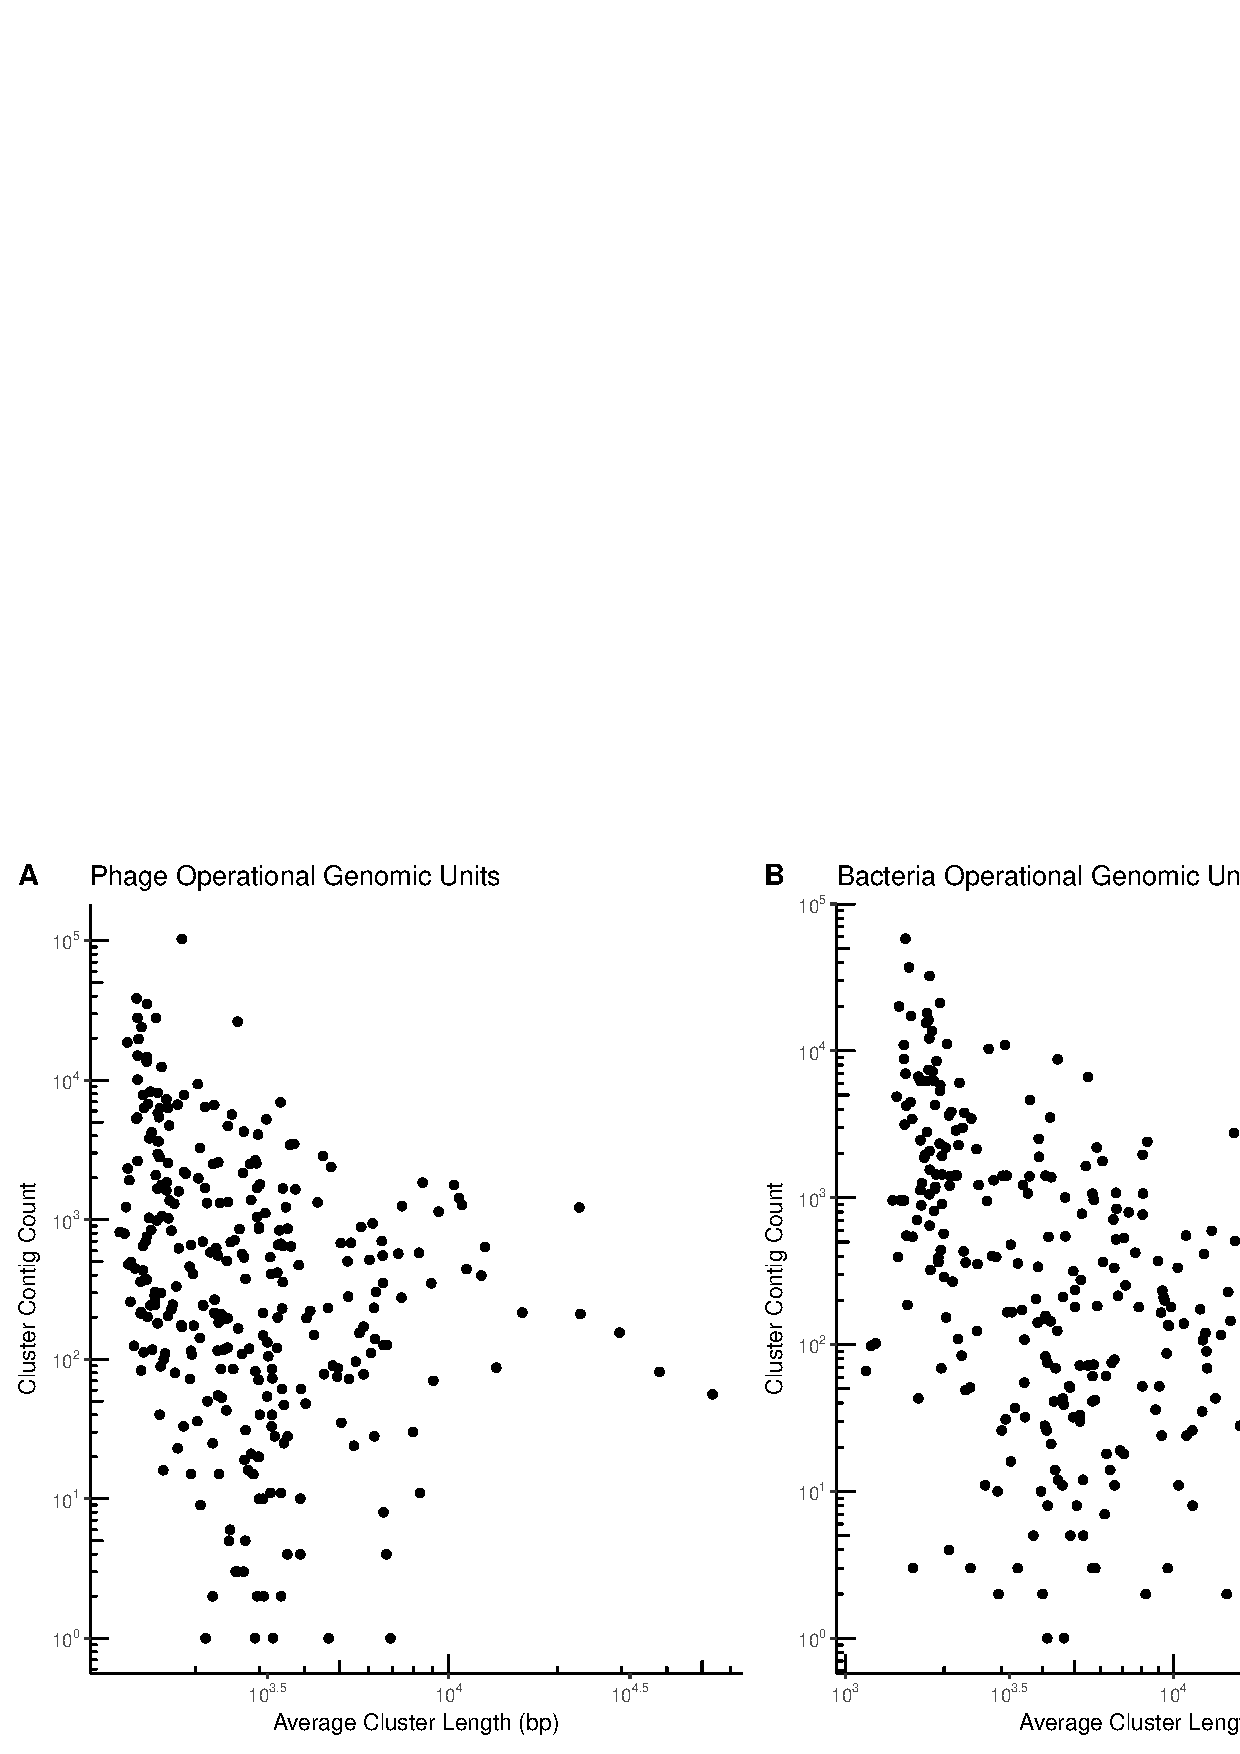
\includegraphics[width=0.80000\textwidth]{../figures/ClusterStats.pdf}
\caption{\textbf{Operational Genomic Unit Summary Statistics.}
\emph{Scatter plot with operational genomic unit clusters organized by
average contig length within the cluster on the x-axis and the number of
contigs in the cluster on the y-axis. Operational genomic units of (A)
bacteriophages and (B) bacteria are shown.}\label{ClusterStats}}
\end{figure}

\newpage

\begin{figure}[htbp]
\centering
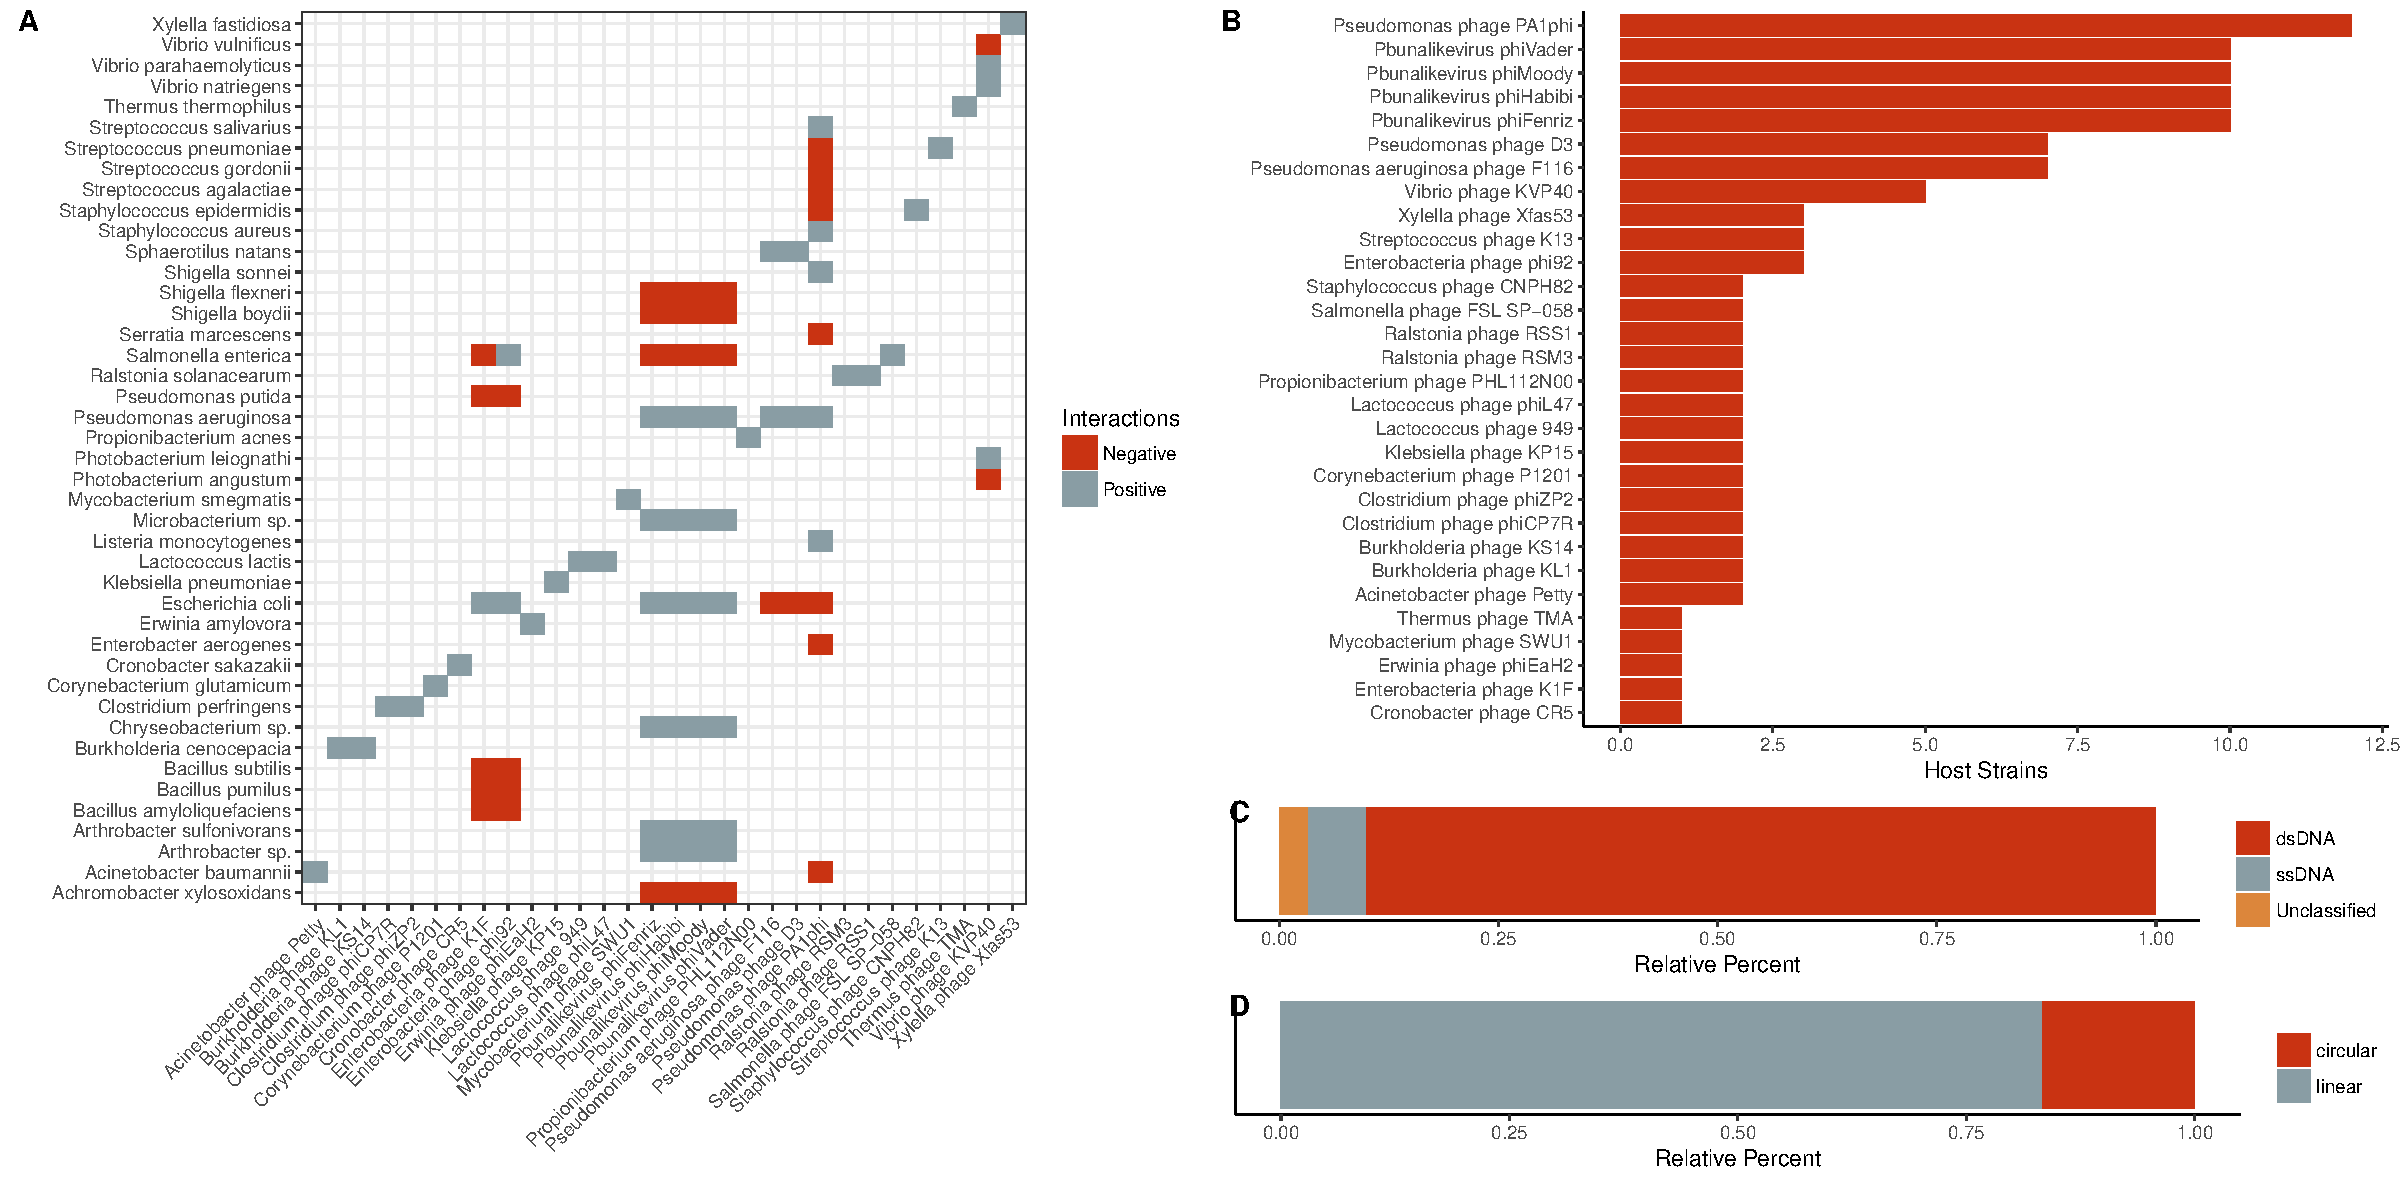
\includegraphics[width=1.00000\textwidth]{../figures/BenchmarkDataset.pdf}
\caption{\textbf{Summary information of validation dataset used in the
interaction predictive model.} \emph{A) Categorical heat-map
highlighting the experimentally validated positive and negative
interactions. Only bacteria species are shown, which represent multiple
reference strains. Phages are labeled on the x-axis and bacteria are
labeled on the y-axis. B) Quantification of bacterial host strains known
to exist for each phage. C) Genome strandedness and D) linearity of the
phage reference genomes used for the
dataset.}\label{ValidationOverview}}
\end{figure}

\newpage

\begin{figure}[htbp]
\centering
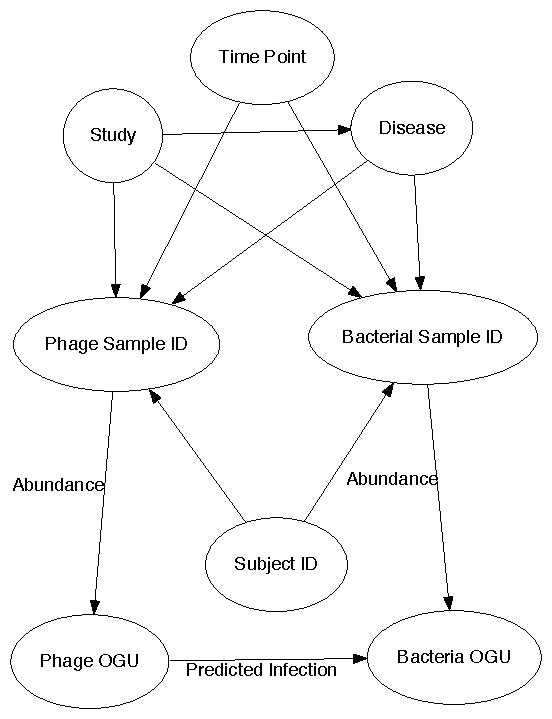
\includegraphics[width=0.50000\textwidth]{../figures/graphdatabasediagram.pdf}
\caption{\textbf{Structure of the interactive network.} \emph{Metadata
relationships to samples (Phage Sample ID and Bacteria Sample ID)
included the associated time point, the study, the subject the sample
was taken from, and the associated disease. Infectious interactions were
recorded between phage and bacteria operational genomic units (OGUs).
Sequence count abundance for each OGU within each sample was also
recorded.}\label{NetworkDiagram}}
\end{figure}

\newpage

\begin{figure}[htbp]
\centering
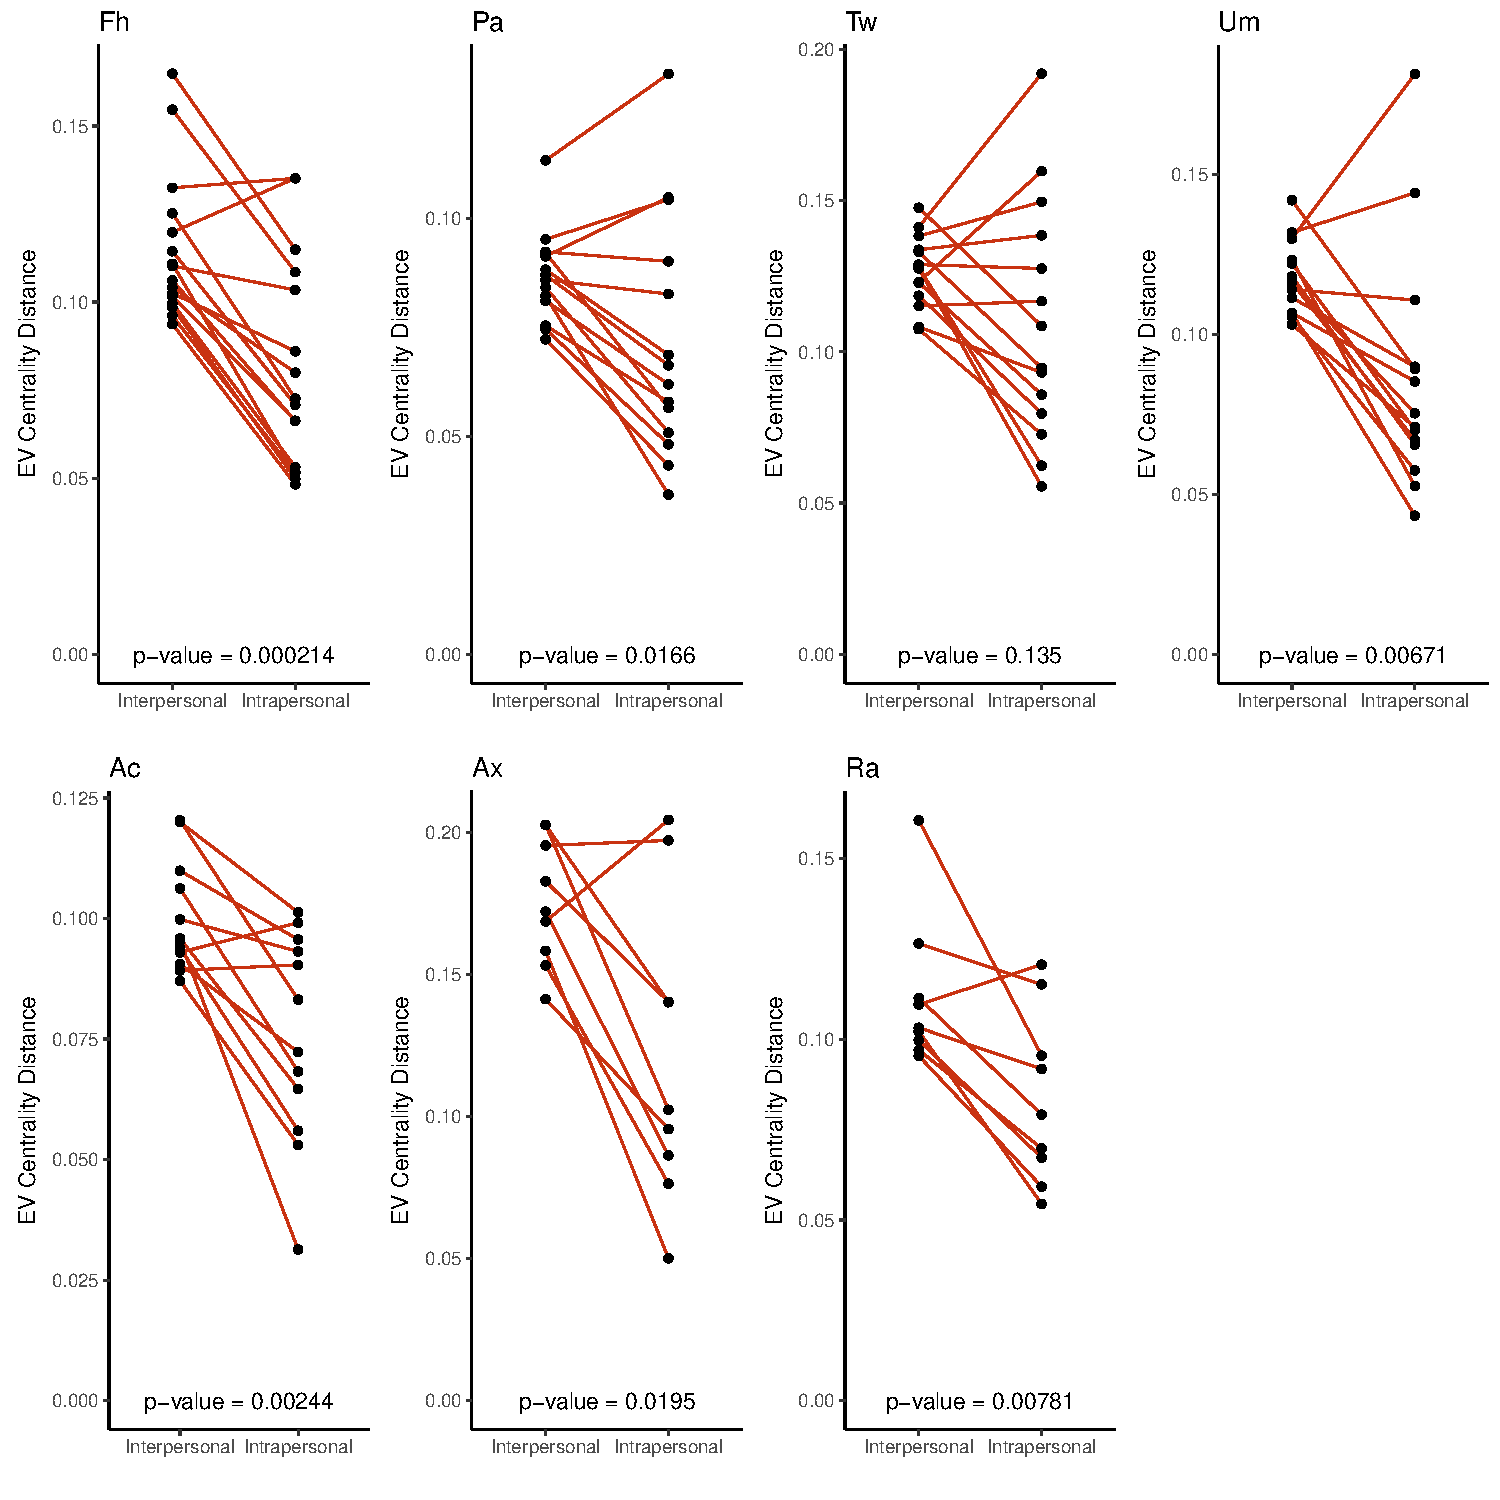
\includegraphics[width=0.75000\textwidth]{../figures/intraallskin.pdf}
\caption{\textbf{Intrapersonal vs Interpersonal Dissimilarity of the
Skin.} \emph{Quantification of skin network dissimilarity within the
same subject and anatomical location over time (intrapersonal) and the
mean dissimilarity between the subject of interest and all other
subjects at the same time and the same anatomical location
(interpersonal), separated by each anatomical site (forehead {[}Fh{]},
palm {[}Pa{]}, toe web {[}Tw{]}, umbilicus {[}Um{]}, antecubital fossa
{[}Ac{]}, axilla {[}Ax{]}, and retroauricular crease {[}Ra{]}). P-value
was calculated using a paired Wilcoxon test.}\label{allskin}}
\end{figure}

\newpage

\section*{References}\label{references}
\addcontentsline{toc}{section}{References}

\hypertarget{refs}{}
\hypertarget{ref-Hannigan:2013im}{}
1. Hannigan GD, Grice EA. Microbial Ecology of the Skin in the Era of
Metagenomics and Molecular Microbiology. Cold Spring Harbor Perspectives
in Medicine. 2013;3: a015362--a015362.

\hypertarget{ref-Hannigan:2014be}{}
2. Hannigan GD, Hodkinson BP, McGinnis K, Tyldsley AS, Anari JB, Horan
AD, et al. Culture-independent pilot study of microbiota colonizing open
fractures and association with severity, mechanism, location, and
complication from presentation to early outpatient follow-up. Journal of
Orthopaedic Research. 2014;32: 597--605.

\hypertarget{ref-Loesche:2016ev}{}
3. Loesche M, Gardner SE, Kalan L, Horwinski J, Zheng Q, Hodkinson BP,
et al. Temporal stability in chronic wound microbiota is associated with
poor healing. Journal of Investigative Dermatology. 2016;

\hypertarget{ref-He:2016ch}{}
4. He Q, Li X, Liu C, Su L, Xia Z, Li X, et al. Dysbiosis of the fecal
microbiota in the TNBS-induced Crohn's disease mouse model. Applied
Microbiology and Biotechnology. 2016; 1--10.

\hypertarget{ref-Norman:2015kb}{}
5. Norman JM, Handley SA, Baldridge MT, Droit L, Liu CY, Keller BC, et
al. Disease-specific alterations in the enteric virome in inflammatory
bowel disease. Cell. 2015;160: 447--460.

\hypertarget{ref-Seekatz:2016fz}{}
6. Seekatz AM, Rao K, Santhosh K, Young VB. Dynamics of the fecal
microbiome in patients with recurrent and nonrecurrent Clostridium
difficile infection. Genome medicine. 2016;8: 47.

\hypertarget{ref-Zackular:2014fba}{}
7. Zackular JP, Rogers MAM, Ruffin MT, Schloss PD. The human gut
microbiome as a screening tool for colorectal cancer. Cancer prevention
research (Philadelphia, Pa). 2014;7: 1112--1121.

\hypertarget{ref-Baxter:2014hb}{}
8. Baxter NT, Zackular JP, Chen GY, Schloss PD. Structure of the gut
microbiome following colonization with human feces determines colonic
tumor burden. Microbiome. 2014;2: 20.

\hypertarget{ref-Manrique:2016dx}{}
9. Manrique P, Bolduc B, Walk ST, Oost J van der, Vos WM de, Young MJ.
Healthy human gut phageome. Proceedings of the National Academy of
Sciences of the United States of America. 2016; 201601060.

\hypertarget{ref-Ly:2014ew}{}
10. Ly M, Abeles SR, Boehm TK, Robles-Sikisaka R, Naidu M,
Santiago-Rodriguez T, et al. Altered Oral Viral Ecology in Association
with Periodontal Disease. mBio. 2014;5: e01133--14--e01133--14.

\hypertarget{ref-Modi:2013fia}{}
11. Modi SR, Lee HH, Spina CS, Collins JJ. Antibiotic treatment expands
the resistance reservoir and ecological network of the phage metagenome.
Nature. 2013;499: 219--222.

\hypertarget{ref-Monaco:2016ita}{}
12. Monaco CL, Gootenberg DB, Zhao G, Handley SA, Ghebremichael MS, Lim
ES, et al. Altered Virome and Bacterial Microbiome in Human
Immunodeficiency Virus-Associated Acquired Immunodeficiency Syndrome.
Cell Host and Microbe. 2016;19: 311--322.

\hypertarget{ref-Hannigan:2015fz}{}
13. Hannigan GD, Meisel JS, Tyldsley AS, Zheng Q, Hodkinson BP,
SanMiguel AJ, et al. The Human Skin Double-Stranded DNA Virome:
Topographical and Temporal Diversity, Genetic Enrichment, and Dynamic
Associations with the Host Microbiome. mBio. 2015;6: e01578--15.

\hypertarget{ref-Minot:2011ez}{}
14. Minot S, Sinha R, Chen J, Li H, Keilbaugh SA, Wu GD, et al. The
human gut virome: Inter-individual variation and dynamic response to
diet. Genome Research. 2011;21: 1616--1625.

\hypertarget{ref-SantiagoRodriguez:2015gd}{}
15. Santiago-Rodriguez TM, Ly M, Bonilla N, Pride DT. The human urine
virome in association with urinary tract infections. Frontiers in
Microbiology. 2015;6: 14.

\hypertarget{ref-Abeles:2015dy}{}
16. Abeles SR, Ly M, Santiago-Rodriguez TM, Pride DT. Effects of Long
Term Antibiotic Therapy on Human Oral and Fecal Viromes. PLOS ONE.
2015;10: e0134941.

\hypertarget{ref-Abeles:2014kj}{}
17. Abeles SR, Robles-Sikisaka R, Ly M, Lum AG, Salzman J, Boehm TK, et
al. Human oral viruses are personal, persistent and gender-consistent.
2014; 1--15.

\hypertarget{ref-Haerter:2014ii}{}
18. Haerter JO, Mitarai N, Sneppen K. Phage and bacteria support mutual
diversity in a narrowing staircase of coexistence. The ISME Journal.
2014;8: 2317--2326.

\hypertarget{ref-Lindell:2005gz}{}
19. Lindell D, Jaffe JD, Johnson ZI, Church GM, Chisholm SW.
Photosynthesis genes in marine viruses yield proteins during host
infection. Nature. 2005;438: 86--89.

\hypertarget{ref-Tyler:2013fl}{}
20. Tyler JS, Beeri K, Reynolds JL, Alteri CJ, Skinner KG, Friedman JH,
et al. Prophage induction is enhanced and required for renal disease and
lethality in an EHEC mouse model. PLoS Pathogens. 2013;9: e1003236.

\hypertarget{ref-Hargreaves:2014ja}{}
21. Hargreaves KR, Kropinski AM, Clokie MR. Bacteriophage behavioral
ecology: How phages alter their bacterial host's habits. Bacteriophage.
2014;4: e29866.

\hypertarget{ref-Moon:2015fa}{}
22. Moon BY, Park JY, Hwang SY, Robinson DA, Thomas JC, Fitzgerald JR,
et al. Phage-mediated horizontal transfer of a Staphylococcus aureus
virulence-associated genomic island. Scientific Reports. 2015;5: 9784.

\hypertarget{ref-Modi:2013fi}{}
23. Modi SR, Lee HH, Spina CS, Collins JJ. Antibiotic treatment expands
the resistance reservoir and ecological network of the phage metagenome.
Nature. 2013;499: 219--222.

\hypertarget{ref-Ogg:1981th}{}
24. Ogg JE, Timme TL, Alemohammad MM. General Transduction in Vibrio
cholerae. Infection and Immunity. 1981;31: 737--741.

\hypertarget{ref-Frost:2005dn}{}
25. Frost LS, Leplae R, Summers AO, Toussaint A. Mobile genetic
elements: the agents of open source evolution. Nature Reviews
Microbiology. 2005;3: 722--732.

\hypertarget{ref-Koskella:2014ds}{}
26. Koskella B, Brockhurst MA. Bacteria-phage coevolution as a driver of
ecological and evolutionary processes in microbial communities. FEMS
Microbiology Reviews. 2014;38: 916--931.

\hypertarget{ref-Jover:2014gq}{}
27. Jover LF, Effler TC, Buchan A, Wilhelm SW, Weitz JS. The elemental
composition of virus particles: implications for marine biogeochemical
cycles. Nature Reviews Microbiology. 2014;12: 519--528.

\hypertarget{ref-Harcombe:2005fd}{}
28. Harcombe WR, Bull JJ. Impact of phages on two-species bacterial
communities. Applied and Environmental Microbiology. 2005;71:
5254--5259.

\hypertarget{ref-Middelboe:2001fl}{}
29. Middelboe M, Hagström A, Blackburn N, Sinn B, Fischer U, Borch NH,
et al. Effects of Bacteriophages on the Population Dynamics of Four
Strains of Pelagic Marine Bacteria. Microbial Ecology. 2001;42:
395--406.

\hypertarget{ref-Poisot:2011jc}{}
30. Poisot T, Lepennetier G, Martinez E, Ramsayer J, Hochberg ME.
Resource availability affects the structure of a natural
bacteriabacteriophage community. Biology letters. 2011;7: 201--204.

\hypertarget{ref-Thompson:2012ki}{}
31. Thompson RM, Brose U, Dunne JA, Hall RO, Hladyz S, Kitching RL, et
al. Food webs: reconciling the structure and function of biodiversity.
Trends in ecology \& evolution. 2012;27: 689--697.

\hypertarget{ref-Moebus:1981kp}{}
32. Moebus K, Nattkemper H. Bacteriophage sensitivity patterns among
bacteria isolated from marine waters. Helgoländer Meeresuntersuchungen.
1981;34: 375--385.

\hypertarget{ref-Flores:2013hc}{}
33. Flores CO, Valverde S, Weitz JS. Multi-scale structure and
geographic drivers of cross-infection within marine bacteria and phages.
The ISME Journal. 2013;7: 520--532.

\hypertarget{ref-Poisot:2012fh}{}
34. Poisot T, Canard E, Mouillot D, Mouquet N, Gravel D. The
dissimilarity of species interaction networks. Ecology letters. 2012;15:
1353--1361.

\hypertarget{ref-Poisot071993}{}
35. Poisot T, Stouffer D. How ecological networks evolve. bioRxiv. 2016;

\hypertarget{ref-Flores:2011bh}{}
36. Flores CO, Meyer JR, Valverde S, Farr L, Weitz JS. Statistical
structure of host-phage interactions. Proceedings of the National
Academy of Sciences of the United States of America. 2011;108: E288--97.

\hypertarget{ref-Jover:2015ev}{}
37. Jover LF, Flores CO, Cortez MH, Weitz JS. Multiple regimes of robust
patterns between network structure and biodiversity. Scientific Reports.
2015;5: 17856.

\hypertarget{ref-Reyes:2010cwa}{}
38. Reyes A, Haynes M, Hanson N, Angly FE, Heath AC, Rohwer F, et al.
Viruses in the faecal microbiota of monozygotic twins and their mothers.
Nature. 2010;466: 334--338.

\hypertarget{ref-Turnbaugh:2009ei}{}
39. Turnbaugh PJ, Hamady M, Yatsunenko T, Cantarel BL, Duncan A, Ley RE,
et al. A core gut microbiome in obese and lean twins. Nature. 2009;457:
480--484.

\hypertarget{ref-LimaMendez:2015hw}{}
40. Lima-Mendez G, Faust K, Henry N, Decelle J, Colin S, Carcillo F, et
al. Ocean plankton. Determinants of community structure in the global
plankton interactome. Science. 2015;348: 1262073--1262073.

\hypertarget{ref-Edwards:2015iz}{}
41. Edwards RA, McNair K, Faust K, Raes J, Dutilh BE. Computational
approaches to predict bacteriophage-host relationships. FEMS
Microbiology Reviews. 2015;40: 258--272.

\hypertarget{ref-Roux:2016cc}{}
42. Roux S, Brum JR, Dutilh BE, Sunagawa S, Duhaime MB, Loy A, et al.
Ecogenomics and potential biogeochemical impacts of globally abundant
ocean viruses. Nature. 2016;537: 689--693.

\hypertarget{ref-Grice:2009eea}{}
43. Grice EA, Kong HH, Conlan S, Deming CB, Davis J, Young AC, et al.
Topographical and Temporal Diversity of the Human Skin Microbiome.
Science. 2009;324: 1190--1192.

\hypertarget{ref-Findley:2013jf}{}
44. Findley K, Oh J, Yang J, Conlan S, Deming C, Meyer JA, et al.
Topographic diversity of fungal and bacterial communities in human skin.
Nature. 2013; 1--6.

\hypertarget{ref-Costello:2009im}{}
45. Costello EK, Lauber CL, Hamady M, Fierer N, Gordon JI, Knight R.
Bacterial community variation in human body habitats across space and
time. Science. 2009;326: 1694--1697.

\hypertarget{ref-Consortium:2012iz}{}
46. Consortium THMP. A framework for human microbiome research. Nature.
2012;486: 215--221.

\hypertarget{ref-Jensen:1998vh}{}
47. Jensen EC, Schrader HS, Rieland B, Thompson TL, Lee KW, Nickerson
KW, et al. Prevalence of broad-host-range lytic bacteriophages of
Sphaerotilus natans, Escherichia coli, and Pseudomonas aeruginosa.
Applied and Environmental Microbiology. 1998;64: 575--580.

\hypertarget{ref-Malki:2015tm}{}
48. Malki K, Kula A, Bruder K, Sible E. Bacteriophages isolated from
Lake Michigan demonstrate broad host-range across several bacterial
phyla. Virology. 2015;

\hypertarget{ref-Schwarzer:2012ez}{}
49. Schwarzer D, Buettner FFR, Browning C, Nazarov S, Rabsch W, Bethe A,
et al. A multivalent adsorption apparatus explains the broad host range
of phage phi92: a comprehensive genomic and structural analysis. Journal
of Virology. 2012;86: 10384--10398.

\hypertarget{ref-Kim:2012dh}{}
50. Kim S, Rahman M, Seol SY, Yoon SS, Kim J. Pseudomonas aeruginosa
bacteriophage PA1Ø requires type IV pili for infection and shows broad
bactericidal and biofilm removal activities. Applied and Environmental
Microbiology. 2012;78: 6380--6385.

\hypertarget{ref-Matsuzaki:1992gw}{}
51. Matsuzaki S, Tanaka S, Koga T, Kawata T. A Broad-Host-Range
Vibriophage, KVP40, Isolated from Sea Water. Microbiology and
Immunology. 1992;36: 93--97.

\hypertarget{ref-Orchard:2014hq}{}
52. Orchard S, Ammari M, Aranda B, Breuza L, Briganti L, Broackes-Carter
F, et al. The MIntAct project--IntAct as a common curation platform for
11 molecular interaction databases. Nucleic Acids Research. 2014;42:
D358--63.

\hypertarget{ref-Turnbaugh:2009hf}{}
53. Turnbaugh PJ, Ridaura VK, Faith JJ, Rey FE, Knight R, Gordon JI. The
effect of diet on the human gut microbiome: a metagenomic analysis in
humanized gnotobiotic mice. Science Translational Medicine. 2009;1:
6ra14--6ra14.

\hypertarget{ref-David:2014cl}{}
54. David LA, Maurice CF, Carmody RN, Gootenberg DB, Button JE, Wolfe
BE, et al. Diet rapidly and reproducibly alters the human gut
microbiome. Nature. 2014;505: 559--563.

\hypertarget{ref-Grice:2009ee}{}
55. Grice EA, Kong HH, Conlan S, Deming CB, Davis J, Young AC, et al.
Topographical and Temporal Diversity of the Human Skin Microbiome.
Science. 2009;324: 1190--1192.

\hypertarget{ref-Minot:2013ih}{}
56. Minot S, Bryson A, Chehoud C, Wu GD, Lewis JD, Bushman FD. Rapid
evolution of the human gut virome. Proceedings of the National Academy
of Sciences of the United States of America. 2013;110: 12450--12455.

\hypertarget{ref-Schloss:2005hz}{}
57. Schloss PD, Handelsman J. Introducing DOTUR, a computer program for
defining operational taxonomic units and estimating species richness.
Applied and Environmental Microbiology. 2005;71: 1501--1506.

\hypertarget{ref-Yilmaz:2010jb}{}
58. Yilmaz S, Allgaier M, Hugenholtz P. Multiple displacement
amplification compromises quantitative analysis of metagenomes. Nature
Methods. 2010;7: 943--944.

\hypertarget{ref-Kim:2008to}{}
59. Kim KH, Chang HW, Nam YD, Roh SW. Amplification of uncultured
single-stranded DNA viruses from rice paddy soil. Applied and \ldots{}.
2008;

\hypertarget{ref-Kim:2011hp}{}
60. Kim K-H, Bae J-W. Amplification methods bias metagenomic libraries
of uncultured single-stranded and double-stranded DNA viruses. Applied
and Environmental Microbiology. 2011;77: 7663--7668.

\hypertarget{ref-Minot:2012ed}{}
61. Minot S, Wu GD, Lewis JD, Bushman FD. Conservation of gene cassettes
among diverse viruses of the human gut. PLOS ONE. 2012;7: e42342.

\hypertarget{ref-Deng:2014eb}{}
62. Deng L, Ignacio-Espinoza JC, Gregory AC, Poulos BT, Weitz JS,
Hugenholtz P, et al. Viral tagging reveals discrete populations in
Synechococcus viral genome sequence space. Nature. 2014;513: 242--245.

\hypertarget{ref-Brum:2015iaa}{}
63. Brum JR, Ignacio-Espinoza JC, Roux S, Doulcier G, Acinas SG, Alberti
A, et al. Ocean plankton. Patterns and ecological drivers of ocean viral
communities. Science. 2015;348: 1261498--1261498.

\hypertarget{ref-Polz:2006fi}{}
64. Polz MF, Hunt DE, Preheim SP, Weinreich DM. Patterns and mechanisms
of genetic and phenotypic differentiation in marine microbes.
Philosophical Transactions of the Royal Society B: Biological Sciences.
2006;361: 2009--2021.

\hypertarget{ref-Gregory:2016cg}{}
65. Gregory AC, Solonenko SA, Ignacio-Espinoza JC, LaButti K, Copeland
A, Sudek S, et al. Genomic differentiation among wild cyanophages
despite widespread horizontal gene transfer. BMC Genomics. 2016;17: 930.

\hypertarget{ref-Grice:2011gy}{}
66. Grice EA, Segre JA. The skin microbiome. Nature Reviews
Microbiology. 2011;9: 244--253.

\hypertarget{ref-Round:2009bz}{}
67. Round JL, Mazmanian SK. The gut microbiota shapes intestinal immune
responses during health and disease. Nature reviews Immunology. 2009;9:
313--323.

\hypertarget{ref-FASTXToolkit:wr}{}
68. Hannon GJ. FASTX-Toolkit.: GNU Affero General Public License.

\hypertarget{ref-Li:2016kd}{}
69. Li D, Luo R, Liu C-M, Leung C-M, Ting H-F, Sadakane K, et al.
MEGAHIT v1.0: A fast and scalable metagenome assembler driven by
advanced methodologies and community practices. METHODS. 2016;102:
3--11.

\hypertarget{ref-Langmead:2012jh}{}
70. Langmead B, Salzberg SL. Fast gapped-read alignment with Bowtie 2.
Nature Methods. 2012;9: 357--359.

\hypertarget{ref-Alneberg:2014fc}{}
71. Alneberg J, Bjarnason BS aacute ri, Bruijn I de, Schirmer M, Quick
J, Ijaz UZ, et al. Binning metagenomic contigs by coverage and
composition. Nature Methods. 2014; 1--7.

\hypertarget{ref-Hyatt:2012cy}{}
72. Hyatt D, LoCascio PF, Hauser LJ, Uberbacher EC. Gene and translation
initiation site prediction in metagenomic sequences. Bioinformatics.
2012;28: 2223--2230.

\hypertarget{ref-caretClassificatio:ux5fU2Litux5f1}{}
73. Kuhn M. caret: Classification and Regression Training.

\hypertarget{ref-Edgar:2007bh}{}
74. Edgar RC. PILER-CR: fast and accurate identification of CRISPR
repeats. BMC Bioinformatics. 2007;8: 18.

\hypertarget{ref-Camacho:2009fc}{}
75. Camacho C, Coulouris G, Avagyan V, Ma N, Papadopoulos J, Bealer K,
et al. BLAST+: architecture and applications. BMC Bioinformatics.
2009;10: 1.

\hypertarget{ref-Buchfink:2015ki}{}
76. Buchfink B, Xie C, Huson DH. Fast and sensitive protein alignment
using DIAMOND. Nature Methods. 2015;12: 59--60.

\hypertarget{ref-Neoj:Fuwr6PBN}{}
77. Neo4j.

\hypertarget{ref-Theigraphsoftware:vh}{}
78. Csardi G, Nepusz T. The igraph software package for complex network
research.

\end{document}
